\documentclass{beamer}
\usetheme{ttuStatsCamp}
\usefonttheme{serif}
\usepackage[T1]{fontenc}
\usepackage[utf8]{inputenc}
\usepackage{url}
\usepackage{graphicx}
\usepackage{setspace}
\usepackage[natbibapa]{apacite}
\usepackage{color}
\usepackage{amsmath}
\usepackage{amsfonts}
\usepackage{Sweavel}
\usepackage{listings}
\usepackage{fancybox}

\def\Sweavesize{\scriptsize}
\def\Rcolor{\color{black}}
%\def\Routcolor{\color{red}}
\def\Rcommentcolor{\color{violet}}
\def\Rbackground{\color[gray]{0.85}}
\def\Routbackground{\color[gray]{0.85}}

\lstset{tabsize=2, breaklines=true, style=Rstyle}



\newcommand{\red}[0]{\textcolor{red}}
\newcommand{\green}[0]{\textcolor{green}}
\newcommand{\blue}[0]{\textcolor{blue}}
\newcommand{\comment}[1]{}
\newcommand{\va}[0]{\vspace{12pt}}
\newcommand{\vb}[0]{\vspace{6pt}}
\newcommand{\vc}[0]{\vspace{3pt}}
\newcommand{\vx}[1]{\vspace{#1pt}}

\title[Lecture 9]{Lecture 9: Moderation Wrap-Up}

\author{Kyle M. Lang}

\institute[TTU IMMAP]{
  Institute for Measurement, Methodology, Analysis \& Policy\\
  Texas Tech University\\
  Lubbock, TX
}

\date{2016 Stats Camp}

\setbeamertemplate{frametitle continuation}{}

\begin{document}

\setkeys{Gin}{width=\textwidth}

\input{sweaveFiles/-001}


\begin{frame}[plain]
  
  \titlepage
  
\end{frame}



\begin{frame}{Outline}

  \begin{itemize}
  \item Multiple Moderators
    \va
  \item Moderated Moderation
    \va
  \item Categorical Moderation
    \va
  \item Multiple Group Modeling
  \end{itemize}

\end{frame}



\begin{frame}{Starting Point}

  So far, we've been looking at this type of model:

  \begin{figure}
    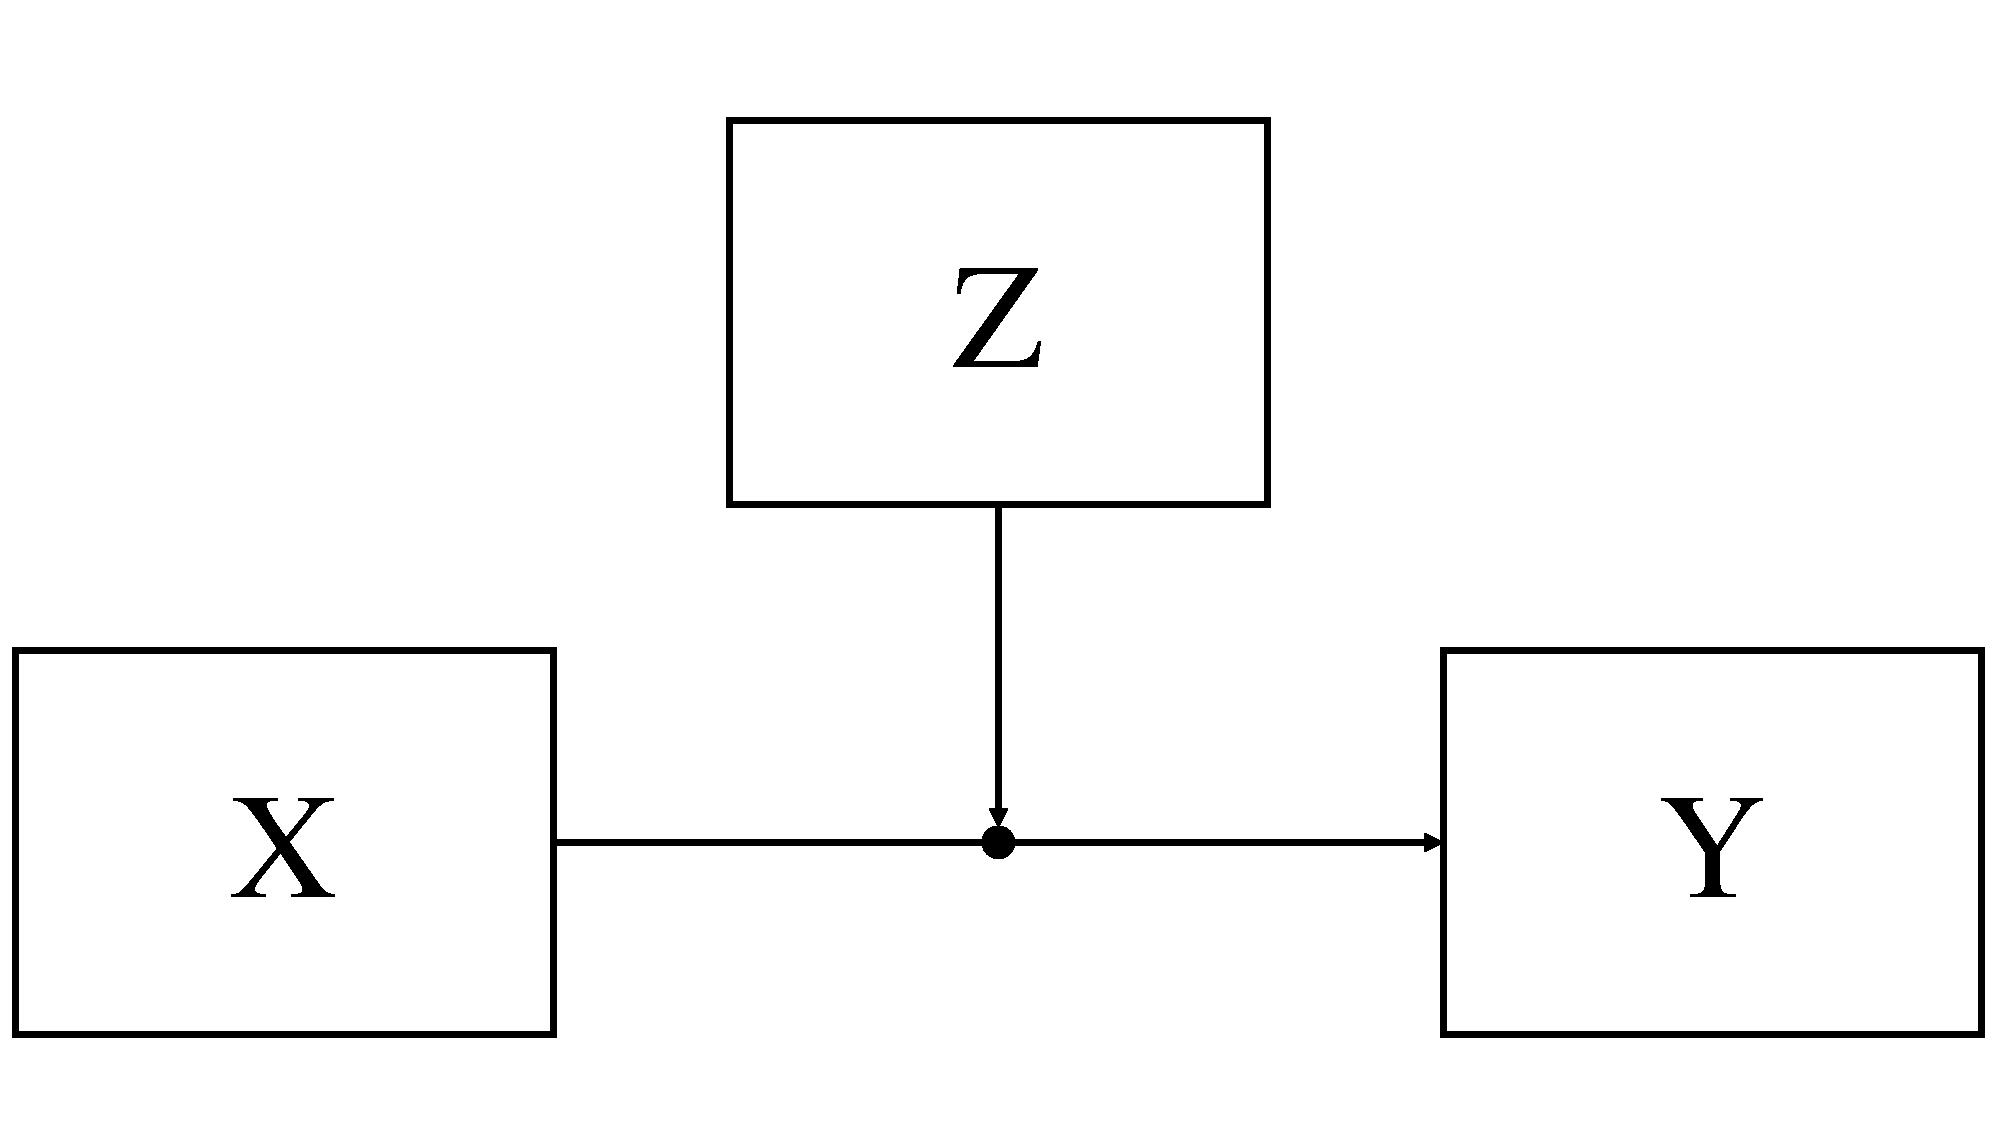
\includegraphics[width=0.7\textwidth]{figures/simpleConceptual.pdf}
  \end{figure}

  We've had one focal variable and one moderator.
  \begin{itemize}
    \item We've been asking questions about how the focal effect
      changes as a function of the moderator.
    \item There's no reason we need to restrict ourselves to a single
      moderator.
  \end{itemize}
  
\end{frame}



\begin{frame}{Multiple Moderation}
  
  Maybe we suspect that the focal effect changes as a function of two other variables.
  \begin{itemize}
    \item We could fit this type of model:
  \end{itemize}

  \begin{figure}
    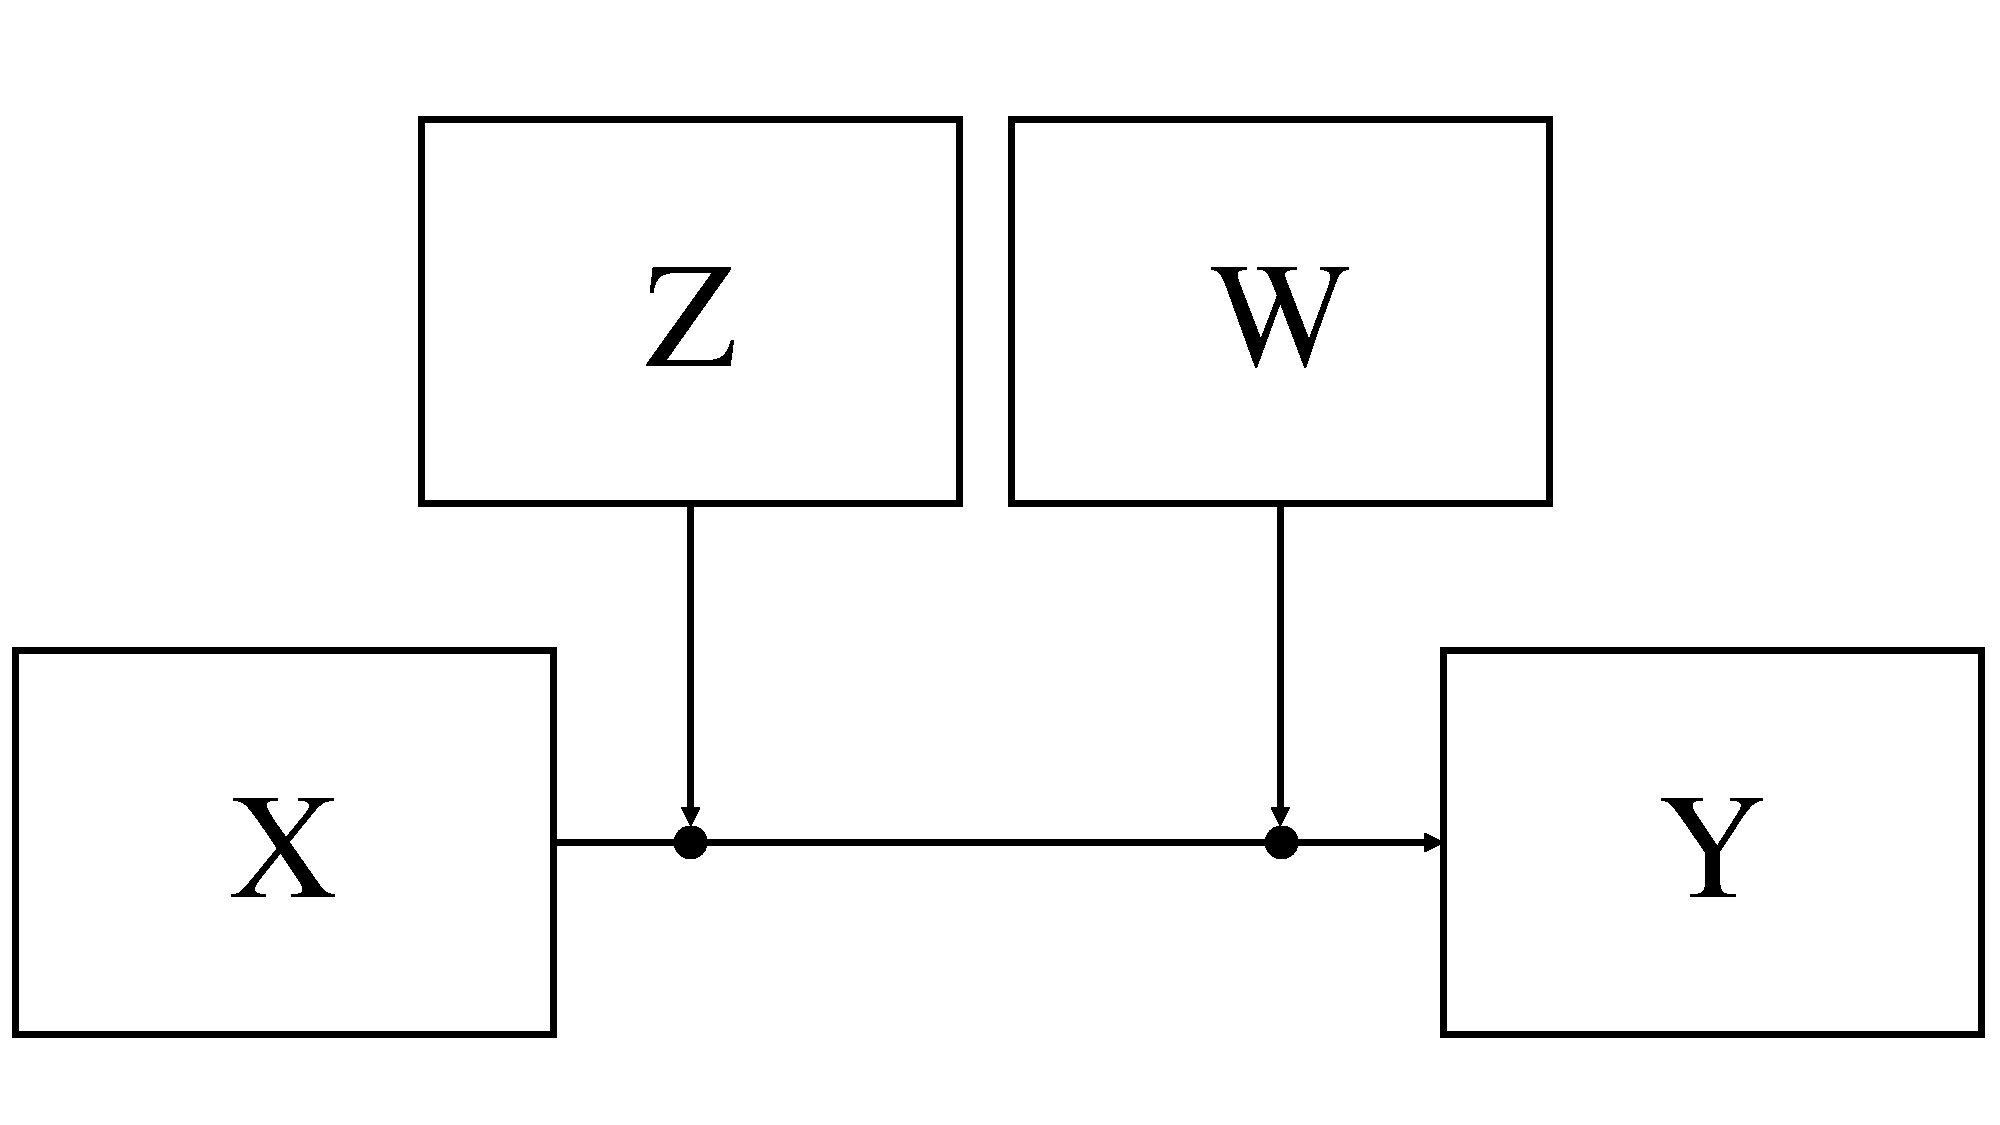
\includegraphics[width=0.7\textwidth]{figures/twoModConceptual.pdf}
  \end{figure}

  Now, the focal effect of $X$ on $Y$ changes as a function of both
  $Z$ and $W$.
  
\end{frame}


\begin{frame}{Multiple Moderation}
  
  The preceding diagram implies the following formula:
  \begin{align*}
    Y = \alpha + f(Z, W) X + \beta_2Z + \beta_3W + e,
  \end{align*}\\
  \va 
  Taking $f(Z, W)$ to be the following simple slope:
  \begin{align*}
    f(Z, W) = \beta_1 + \beta_4Z + \beta_5W
  \end{align*}\\
  \va 
  Produces the following analytic equation:
  \begin{align*}
    Y = \alpha + \beta_1X + \beta_2Z + \beta_3W + \beta_4XZ + \beta_5XW + e
  \end{align*}\\
  \va
  We can easily fit this model in any regression software
  \vb
  \begin{itemize}
  \item We can test for significant moderating effects of $Z$ and $W$
    by testing for non-zero $\beta_4$ and $\beta_5$, respectively.
  \end{itemize}
  
\end{frame}



\begin{frame}{Multiple Moderation}
  
  Our analytic diagram is predictably extended:

  \begin{figure}
    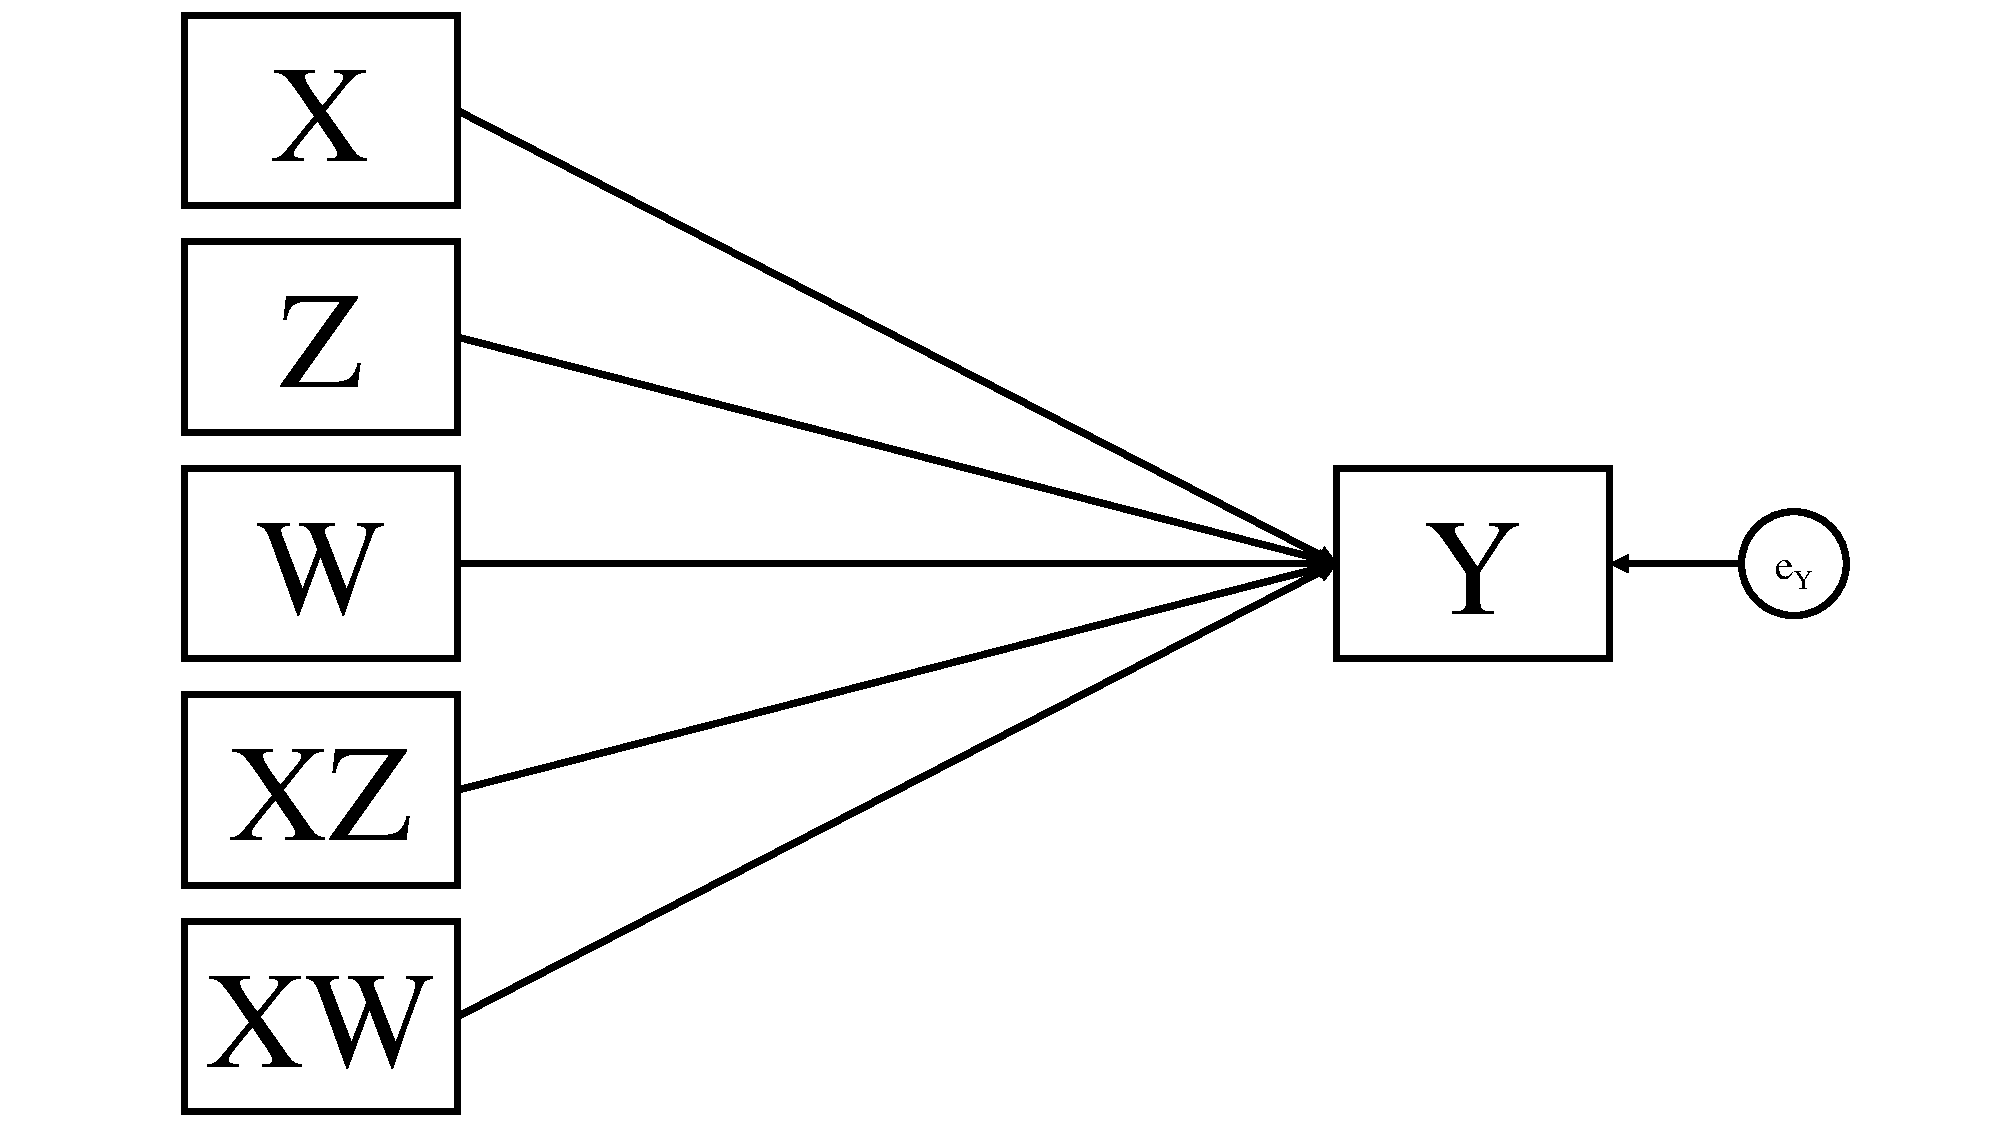
\includegraphics[width=\textwidth]{figures/twoModAnalytic.pdf}
  \end{figure}

\end{frame}

  

\begin{frame}[allowframebreaks]{Example}
    
\begin{Schunk}
\begin{Sinput}
 library(lavaan)
 dataDir <- "../data/"
 dat1 <- readRDS(paste0(dataDir, "adamsKlpsData.rds"))
 ## Specify the CFA model:
 mod1.1 <- "
 merit =~ meritP1 + meritP2 + meritP3
 policy =~ policyP1 + policyP2 + policyP3
 "
 ## Fit the CFA and check model:
 out1.1 <- cfa(mod1.1, data = dat1, std.lv = TRUE)
 ## Check model fit:
 round(fitMeasures(out1.1)[c("chisq", "df", "pvalue", "cfi", 
                             "tli", "rmsea", "srmr")], 4)
\end{Sinput}
\begin{Soutput}
  chisq      df  pvalue     cfi     tli   rmsea    srmr 
16.8695  8.0000  0.0315  0.9215  0.8529  0.1129  0.0653 
\end{Soutput}
\begin{Sinput}
 summary(out1.1)
\end{Sinput}
\begin{Soutput}
lavaan (0.5-20) converged normally after  22 iterations

  Number of observations                            87

  Estimator                                         ML
  Minimum Function Test Statistic               16.869
  Degrees of freedom                                 8
  P-value (Chi-square)                           0.031

Parameter Estimates:

  Information                                 Expected
  Standard Errors                             Standard

Latent Variables:
                   Estimate  Std.Err  Z-value  P(>|z|)
  merit =~                                            
    meritP1           0.690    0.134    5.155    0.000
    meritP2           0.968    0.142    6.830    0.000
    meritP3           0.748    0.137    5.458    0.000
  policy =~                                           
    policyP1          0.851    0.186    4.570    0.000
    policyP2          0.996    0.167    5.967    0.000
    policyP3          1.121    0.177    6.339    0.000

Covariances:
                   Estimate  Std.Err  Z-value  P(>|z|)
  merit ~~                                            
    policy           -0.336    0.131   -2.563    0.010

Variances:
                   Estimate  Std.Err  Z-value  P(>|z|)
    meritP1           0.865    0.165    5.248    0.000
    meritP2           0.445    0.201    2.211    0.027
    meritP3           0.833    0.172    4.857    0.000
    policyP1          1.836    0.324    5.671    0.000
    policyP2          0.942    0.256    3.683    0.000
    policyP3          0.857    0.297    2.882    0.004
    merit             1.000                           
    policy            1.000                           
\end{Soutput}
\end{Schunk}


\pagebreak

\begin{Schunk}
\begin{Sinput}
 round(fitMeasures(out1)[c("chisq", "df", "pvalue", "cfi", 
                           "tli", "rmsea", "srmr")], 3)
\end{Sinput}
\begin{Soutput}
 chisq     df pvalue    cfi    tli  rmsea   srmr 
41.021 24.000  0.017  0.987  0.981  0.038  0.026 
\end{Soutput}
\end{Schunk}


\pagebreak

\begin{Schunk}
\begin{Sinput}
 mod3 <- "
 att3 ~ att2 + b2*conf2 + cp2*horn2
 att2 ~ att1 + b1*conf1 + cp1*horn1
 
 conf3 ~ conf2 + a2*horn2
 conf2 ~ conf1 + a1*horn1
 
 horn3 ~ horn2
 horn2 ~ horn1
 
 horn3 ~~ conf3 + att3
 conf3 ~~ att3
 
 horn2 ~~ conf2 + att2
 conf2 ~~ att2
 
 a1 == a2
 b1 == b2
 cp1 == cp2
 "
 out3 <- sem(mod3, data = dat1)
 summary(out3)
\end{Sinput}
\begin{Soutput}
lavaan (0.5-20) converged normally after  46 iterations

  Number of observations                           500

  Estimator                                         ML
  Minimum Function Test Statistic              294.220
  Degrees of freedom                                18
  P-value (Chi-square)                           0.000

Parameter Estimates:

  Information                                 Expected
  Standard Errors                             Standard

Regressions:
                   Estimate  Std.Err  Z-value  P(>|z|)
  att3 ~                                              
    att2              0.497    0.035   14.234    0.000
    conf2     (b2)    0.098    0.019    5.200    0.000
    horn2    (cp2)    0.083    0.072    1.157    0.247
  att2 ~                                              
    att1              0.530    0.040   13.345    0.000
    conf1     (b1)    0.098    0.019    5.200    0.000
    horn1    (cp1)    0.083    0.072    1.157    0.247
  conf3 ~                                             
    conf2             0.684    0.035   19.602    0.000
    horn2     (a2)    0.493    0.107    4.596    0.000
  conf2 ~                                             
    conf1             0.623    0.032   19.546    0.000
    horn1     (a1)    0.493    0.107    4.596    0.000
  horn3 ~                                             
    horn2             0.826    0.030   27.609    0.000
  horn2 ~                                             
    horn1             0.714    0.024   29.181    0.000

Covariances:
                   Estimate  Std.Err  Z-value  P(>|z|)
  conf3 ~~                                            
    horn3             1.016    0.155    6.556    0.000
  att3 ~~                                             
    horn3             0.322    0.093    3.483    0.000
    conf3             3.574    0.465    7.691    0.000
  conf2 ~~                                            
    horn2             0.836    0.124    6.721    0.000
  att2 ~~                                             
    horn2             0.273    0.083    3.289    0.001
    conf2             2.027    0.400    5.067    0.000

Variances:
                   Estimate  Std.Err  Z-value  P(>|z|)
    att3              6.019    0.381   15.811    0.000
    att2              6.041    0.382   15.811    0.000
    conf3            15.814    1.000   15.811    0.000
    conf2            12.570    0.795   15.811    0.000
    horn3             0.695    0.044   15.811    0.000
    horn2             0.560    0.035   15.811    0.000

Constraints:
                                               |Slack|
    a1 - (a2)                                    0.000
    b1 - (b2)                                    0.000
    cp1 - (cp2)                                  0.000
\end{Soutput}
\begin{Sinput}
 chiDiff <- fitMeasures(out3)["chisq"] -
     fitMeasures(out1)["chisq"]
 dfDiff <- fitMeasures(out3)["df"] -
     fitMeasures(out1)["df"]
 pchisq(chiDiff, dfDiff, lower = FALSE)
\end{Sinput}
\begin{Soutput}
     chisq 
0.02684148 
\end{Soutput}
\end{Schunk}


\pagebreak

\begin{Schunk}
\begin{Sinput}
 mod4 <- "
 att3 ~ att2 + b2*conf2 + cp*horn1
 att2 ~ att1 + b1*conf1
 
 conf3 ~ conf2 + a2*horn2
 conf2 ~ conf1 + a1*horn1
 
 att2 + att3 ~ income
 conf2 + conf3 ~ income 
 horn2 + horn3 ~ income
 
 horn3 ~ horn2
 horn2 ~ horn1
 
 horn3 ~~ conf3 + att3
 conf3 ~~ att3
 
 horn2 ~~ conf2 + att2
 conf2 ~~ att2
 
 ab := a1*b2
 "
 out4 <- sem(mod4, data = dat1, se = "boot", boot = nBoot)
 summary(out4)
\end{Sinput}
\begin{Soutput}
lavaan (0.5-20) converged normally after  63 iterations

  Number of observations                           500

  Estimator                                         ML
  Minimum Function Test Statistic              219.789
  Degrees of freedom                                16
  P-value (Chi-square)                           0.000

Parameter Estimates:

  Information                                 Observed
  Standard Errors                            Bootstrap
  Number of requested bootstrap draws             2000
  Number of successful bootstrap draws            2000

Regressions:
                   Estimate  Std.Err  Z-value  P(>|z|)
  att3 ~                                              
    att2              0.513    0.039   13.099    0.000
    conf2     (b2)    0.022    0.027    0.826    0.409
    horn1     (cp)   -0.119    0.084   -1.418    0.156
  att2 ~                                              
    att1              0.477    0.043   10.980    0.000
    conf1     (b1)    0.084    0.028    3.048    0.002
  conf3 ~                                             
    conf2             0.488    0.041   11.803    0.000
    horn2     (a2)    0.492    0.160    3.076    0.002
  conf2 ~                                             
    conf1             0.543    0.037   14.594    0.000
    horn1     (a1)    0.175    0.146    1.204    0.228
  att2 ~                                              
    income            0.052    0.013    4.108    0.000
  att3 ~                                              
    income            0.057    0.012    4.853    0.000
  conf2 ~                                             
    income            0.110    0.016    6.871    0.000
  conf3 ~                                             
    income            0.148    0.018    8.206    0.000
  horn2 ~                                             
    income            0.016    0.003    5.698    0.000
  horn3 ~                                             
    income            0.013    0.004    3.555    0.000
    horn2             0.780    0.033   23.921    0.000
  horn2 ~                                             
    horn1             0.654    0.026   25.525    0.000

Covariances:
                   Estimate  Std.Err  Z-value  P(>|z|)
  conf3 ~~                                            
    horn3             0.915    0.152    6.020    0.000
  att3 ~~                                             
    horn3             0.322    0.092    3.489    0.000
    conf3             2.971    0.412    7.215    0.000
  conf2 ~~                                            
    horn2             0.678    0.112    6.026    0.000
  att2 ~~                                             
    horn2             0.203    0.083    2.428    0.015
    conf2             1.601    0.382    4.194    0.000

Variances:
                   Estimate  Std.Err  Z-value  P(>|z|)
    att3              5.771    0.351   16.431    0.000
    att2              5.821    0.362   16.099    0.000
    conf3            14.066    0.828   16.988    0.000
    conf2            11.512    0.729   15.792    0.000
    horn2             0.529    0.033   16.004    0.000
    horn3             0.677    0.040   16.788    0.000

Defined Parameters:
                   Estimate  Std.Err  Z-value  P(>|z|)
    ab                0.004    0.007    0.559    0.576
\end{Soutput}
\begin{Sinput}
 parameterEstimates(out4, boot = "bca.simple")[ , -c(1 : 3)]
\end{Sinput}
\begin{Soutput}
   label     est    se      z pvalue ci.lower ci.upper
1          0.513 0.039 13.099  0.000    0.438    0.589
2     b2   0.022 0.027  0.826  0.409   -0.030    0.076
3     cp  -0.119 0.084 -1.418  0.156   -0.275    0.051
4          0.477 0.043 10.980  0.000    0.396    0.565
5     b1   0.084 0.028  3.048  0.002    0.029    0.139
6          0.488 0.041 11.803  0.000    0.410    0.569
7     a2   0.492 0.160  3.076  0.002    0.186    0.818
8          0.543 0.037 14.594  0.000    0.464    0.614
9     a1   0.175 0.146  1.204  0.228   -0.099    0.468
10         0.052 0.013  4.108  0.000    0.028    0.077
11         0.057 0.012  4.853  0.000    0.033    0.079
12         0.110 0.016  6.871  0.000    0.079    0.141
13         0.148 0.018  8.206  0.000    0.114    0.183
14         0.016 0.003  5.698  0.000    0.011    0.022
15         0.013 0.004  3.555  0.000    0.005    0.019
16         0.780 0.033 23.921  0.000    0.714    0.844
17         0.654 0.026 25.525  0.000    0.601    0.703
18         0.915 0.152  6.020  0.000    0.633    1.225
19         0.322 0.092  3.489  0.000    0.143    0.508
20         2.971 0.412  7.215  0.000    2.207    3.834
21         0.678 0.112  6.026  0.000    0.466    0.903
22         0.203 0.083  2.428  0.015    0.040    0.369
23         1.601 0.382  4.194  0.000    0.870    2.387
24         5.771 0.351 16.431  0.000    5.130    6.509
25         5.821 0.362 16.099  0.000    5.171    6.590
26        14.066 0.828 16.988  0.000   12.623   15.934
27        11.512 0.729 15.792  0.000   10.207   13.077
28         0.529 0.033 16.004  0.000    0.472    0.602
29         0.677 0.040 16.788  0.000    0.606    0.765
30         1.809 0.000     NA     NA    1.809    1.809
31         1.470 0.000     NA     NA    1.470    1.470
32         3.939 0.000     NA     NA    3.939    3.939
33         5.753 0.000     NA     NA    5.753    5.753
34         8.748 0.000     NA     NA    8.748    8.748
35         8.475 0.000     NA     NA    8.475    8.475
36        16.763 0.000     NA     NA   16.763   16.763
37        28.025 0.000     NA     NA   28.025   28.025
38        39.156 0.000     NA     NA   39.156   39.156
39       136.353 0.000     NA     NA  136.353  136.353
40    ab   0.004 0.007  0.559  0.576   -0.003    0.031
\end{Soutput}
\end{Schunk}


\pagebreak

\begin{Schunk}
\begin{Sinput}
 ## Completely Standardized:
 abCS <- (sdX * ab) / sdY
 abCS
\end{Sinput}
\begin{Soutput}
[1] 0.1345859
\end{Soutput}
\begin{Sinput}
 cPrimeCS <- (sdX * cPrime) / sdY
 cPrimeCS
\end{Sinput}
\begin{Soutput}
       cp 
0.1790413 
\end{Soutput}
\begin{Sinput}
 cCS <- abCS + cPrimeCS
 cCS
\end{Sinput}
\begin{Soutput}
       cp 
0.3136272 
\end{Soutput}
\end{Schunk}


\pagebreak

\begin{Schunk}
\begin{Sinput}
 mod3 <- "
 fX =~ x1 + x2 + x3
 fZ =~ z1 + z2 + z3
 fY =~ y1 + y2 + y3
 fXZ =~ x1z1R + x1z2R + x1z3R +
 x2z1R + x2z2R + x2z3R +
 x3z1R + x3z2R + x3z3R
 
 fY ~ fX + fZ + fXZ
 
 fX ~~ fZ
 fX ~~ 0*fXZ
 fZ ~~ 0*fXZ
 
 x1z1R ~~ x1z2R + x1z3R + x2z1R + x3z1R
 x1z2R ~~ x1z3R + x2z2R + x3z2R
 x1z3R ~~ x2z3R + x3z3R
 
 x2z1R ~~ x2z2R + x2z3R + x3z1R
 x2z2R ~~ x2z3R + x3z2R
 x2z3R ~~ x3z3R
 
 x3z1R ~~ x3z2R + x3z3R
 x3z2R ~~ x3z3R
 "
 out3 <- sem(mod3, data = dat2, std.lv = TRUE)
 summary(out3)
\end{Sinput}
\begin{Soutput}
lavaan (0.5-20) converged normally after  53 iterations

  Number of observations                           500

  Estimator                                         ML
  Minimum Function Test Statistic               74.899
  Degrees of freedom                               113
  P-value (Chi-square)                           0.998

Parameter Estimates:

  Information                                 Expected
  Standard Errors                             Standard

Latent Variables:
                   Estimate  Std.Err  Z-value  P(>|z|)
  fX =~                                               
    x1                0.670    0.043   15.424    0.000
    x2                0.660    0.043   15.256    0.000
    x3                0.704    0.045   15.569    0.000
  fZ =~                                               
    z1                0.738    0.048   15.342    0.000
    z2                0.734    0.048   15.156    0.000
    z3                0.718    0.046   15.602    0.000
  fY =~                                               
    y1                0.396    0.046    8.545    0.000
    y2                0.369    0.044    8.441    0.000
    y3                0.383    0.045    8.558    0.000
  fXZ =~                                              
    x1z1R             0.361    0.053    6.833    0.000
    x1z2R             0.427    0.056    7.615    0.000
    x1z3R             0.432    0.053    8.190    0.000
    x2z1R             0.558    0.056    9.914    0.000
    x2z2R             0.616    0.062   10.008    0.000
    x2z3R             0.520    0.057    9.153    0.000
    x3z1R             0.516    0.059    8.805    0.000
    x3z2R             0.626    0.063   10.007    0.000
    x3z3R             0.521    0.058    8.936    0.000

Regressions:
                   Estimate  Std.Err  Z-value  P(>|z|)
  fY ~                                                
    fX                1.658    0.239    6.930    0.000
    fZ               -0.074    0.099   -0.750    0.453
    fXZ               0.488    0.120    4.049    0.000

Covariances:
                   Estimate  Std.Err  Z-value  P(>|z|)
  fX ~~                                               
    fZ                0.232    0.058    3.987    0.000
    fXZ               0.000                           
  fZ ~~                                               
    fXZ               0.000                           
  x1z1R ~~                                            
    x1z2R             0.273    0.032    8.397    0.000
    x1z3R             0.309    0.033    9.358    0.000
    x2z1R             0.232    0.031    7.566    0.000
    x3z1R             0.235    0.032    7.376    0.000
  x1z2R ~~                                            
    x1z3R             0.231    0.032    7.243    0.000
    x2z2R             0.211    0.035    5.982    0.000
    x3z2R             0.250    0.041    6.163    0.000
  x1z3R ~~                                            
    x2z3R             0.213    0.030    7.010    0.000
    x3z3R             0.213    0.034    6.312    0.000
  x2z1R ~~                                            
    x2z2R             0.247    0.043    5.787    0.000
    x2z3R             0.252    0.040    6.368    0.000
    x3z1R             0.233    0.033    7.103    0.000
  x2z2R ~~                                            
    x2z3R             0.304    0.043    7.086    0.000
    x3z2R             0.199    0.040    5.018    0.000
  x2z3R ~~                                            
    x3z3R             0.139    0.030    4.570    0.000
  x3z1R ~~                                            
    x3z2R             0.212    0.041    5.116    0.000
    x3z3R             0.260    0.040    6.454    0.000
  x3z2R ~~                                            
    x3z3R             0.157    0.041    3.846    0.000

Variances:
                   Estimate  Std.Err  Z-value  P(>|z|)
    x1                0.511    0.042   12.093    0.000
    x2                0.514    0.042   12.221    0.000
    x3                0.548    0.046   11.977    0.000
    z1                0.523    0.052   10.142    0.000
    z2                0.546    0.052   10.444    0.000
    z3                0.461    0.048    9.704    0.000
    y1                0.495    0.043   11.398    0.000
    y2                0.542    0.044   12.334    0.000
    y3                0.444    0.040   11.179    0.000
    x1z1R             0.743    0.050   14.912    0.000
    x1z2R             0.754    0.055   13.682    0.000
    x1z3R             0.694    0.050   13.824    0.000
    x2z1R             0.641    0.057   11.332    0.000
    x2z2R             0.708    0.067   10.575    0.000
    x2z3R             0.671    0.056   12.009    0.000
    x3z1R             0.736    0.060   12.310    0.000
    x3z2R             0.724    0.070   10.277    0.000
    x3z3R             0.707    0.060   11.823    0.000
    fX                1.000                           
    fZ                1.000                           
    fY                1.000                           
    fXZ               1.000                           
\end{Soutput}
\end{Schunk}


\pagebreak

\begin{Schunk}
\begin{Sinput}
 parameterEstimates(out2.1, boot = bootType)[ , -c(1 : 3)]
\end{Sinput}
\begin{Soutput}
     label    est    se      z pvalue ci.lower ci.upper
1       b1 -0.008 0.145 -0.052  0.959   -0.286    0.275
2       b2  0.595 0.142  4.184  0.000    0.317    0.861
3       cp  0.134 0.076  1.763  0.078   -0.019    0.281
4      d21 -0.301 0.110 -2.733  0.006   -0.508   -0.076
5       a2  0.090 0.072  1.253  0.210   -0.073    0.220
6       a1 -0.266 0.061 -4.384  0.000   -0.384   -0.148
7           0.987 0.164  6.013  0.000    0.733    1.390
8           0.689 0.094  7.309  0.000    0.537    0.919
9           0.719 0.112  6.389  0.000    0.535    0.980
10          2.444 0.000     NA     NA    2.444    2.444
11     ab1  0.002 0.040  0.050  0.960   -0.080    0.081
12     ab2  0.053 0.044  1.215  0.225   -0.031    0.146
13  fullIE  0.048 0.026  1.822  0.068    0.012    0.117
14 totalIE  0.103 0.048  2.145  0.032    0.011    0.202
\end{Soutput}
\end{Schunk}

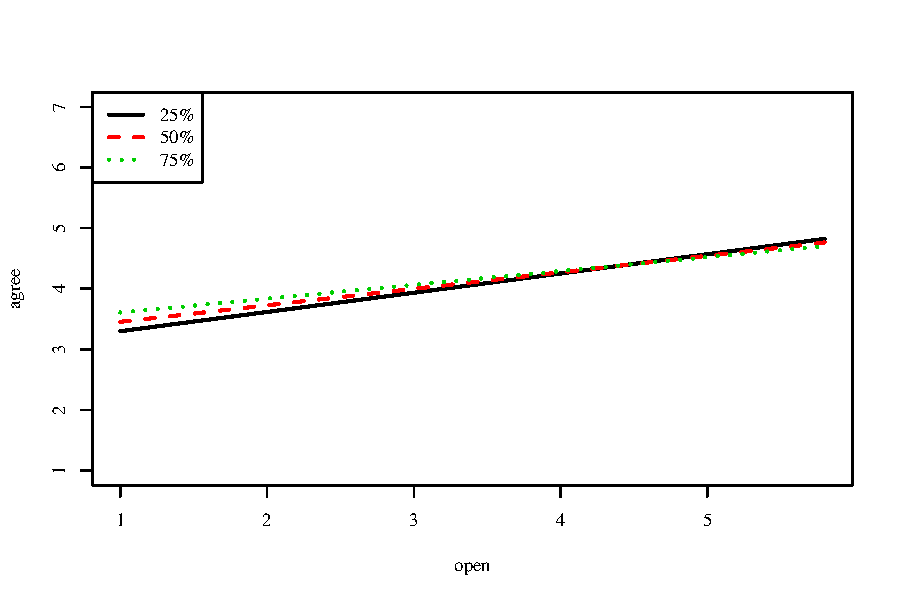
\includegraphics{sweaveFiles/-008}

\pagebreak

\begin{Schunk}
\begin{Sinput}
 ## Possible range of a:
 aMarg <- sqrt(s2M * s2Y - sYM^2) * sqrt(s2X * s2Y - sYX^2)
 aInt <- c(
     (sYM * sYX - aMarg) / (s2X * s2Y),
     (sYM * sYX + aMarg) / (s2X * s2Y)
 )
 aInt
\end{Sinput}
\begin{Soutput}
[1] -0.4378558  0.5793099
\end{Soutput}
\begin{Sinput}
 ##
 ## Possible range of b:
 bMarg <- sqrt(s2X * s2Y - sYX^2) / sqrt(s2X * s2M - sMX^2)
 bInt <- c(-1 * bMarg, bMarg)
 bInt
\end{Sinput}
\begin{Soutput}
[1] -1.289996  1.289996
\end{Soutput}
\begin{Sinput}
 ##
 ## max(a):
 aMax <- ifelse(coef(out2)["a"] < 0,
                aInt[1],
                aInt[2])
 aMax
\end{Sinput}
\begin{Soutput}
        a 
0.5793099 
\end{Soutput}
\begin{Sinput}
 ##
 ## max(b)
 bMax <- ifelse(coef(out2)["b"] < 0,
                bInt[1],
                bInt[2])
 bMax
\end{Sinput}
\begin{Soutput}
       b 
1.289996 
\end{Soutput}
\begin{Sinput}
 ##
 ## max(ab)
 abMax <- aMax * bMax
 abMax
\end{Sinput}
\begin{Soutput}
        a 
0.7473075 
\end{Soutput}
\begin{Sinput}
 ##
 ## Kappa Squared:
 k2 <- ab / abMax
 k2
\end{Sinput}
\begin{Soutput}
        a 
0.1359491 
\end{Soutput}
\end{Schunk}

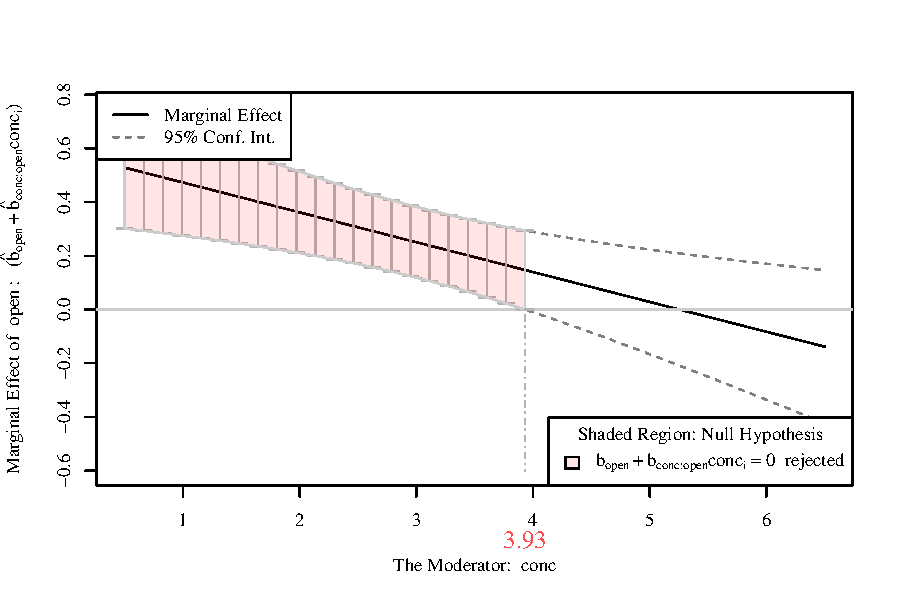
\includegraphics{sweaveFiles/-009}

\end{frame}



\begin{frame}{Moderated Moderation}
  
  The additive two-way interaction model is more flexible than the
  simple single-moderator model, but it still imposes constraints.
  \va
  \begin{itemize}
    \item The moderating effect of $Z$ (or $W$) on the $X \rightarrow
      Y$ relation is assumed to be constant across levels of $W$ (or
      $Z$).
      \vb
    \item I.e., the moderation is not moderated
  \end{itemize}
  
  \va
  We can relax this constraint by modeling moderation of the moderated
  effect using a three-way interaction.
  
\end{frame}



\begin{frame}{Moderated Moderation}
  
  Moderated moderation implies the following conceptual diagram:
  \begin{figure}
    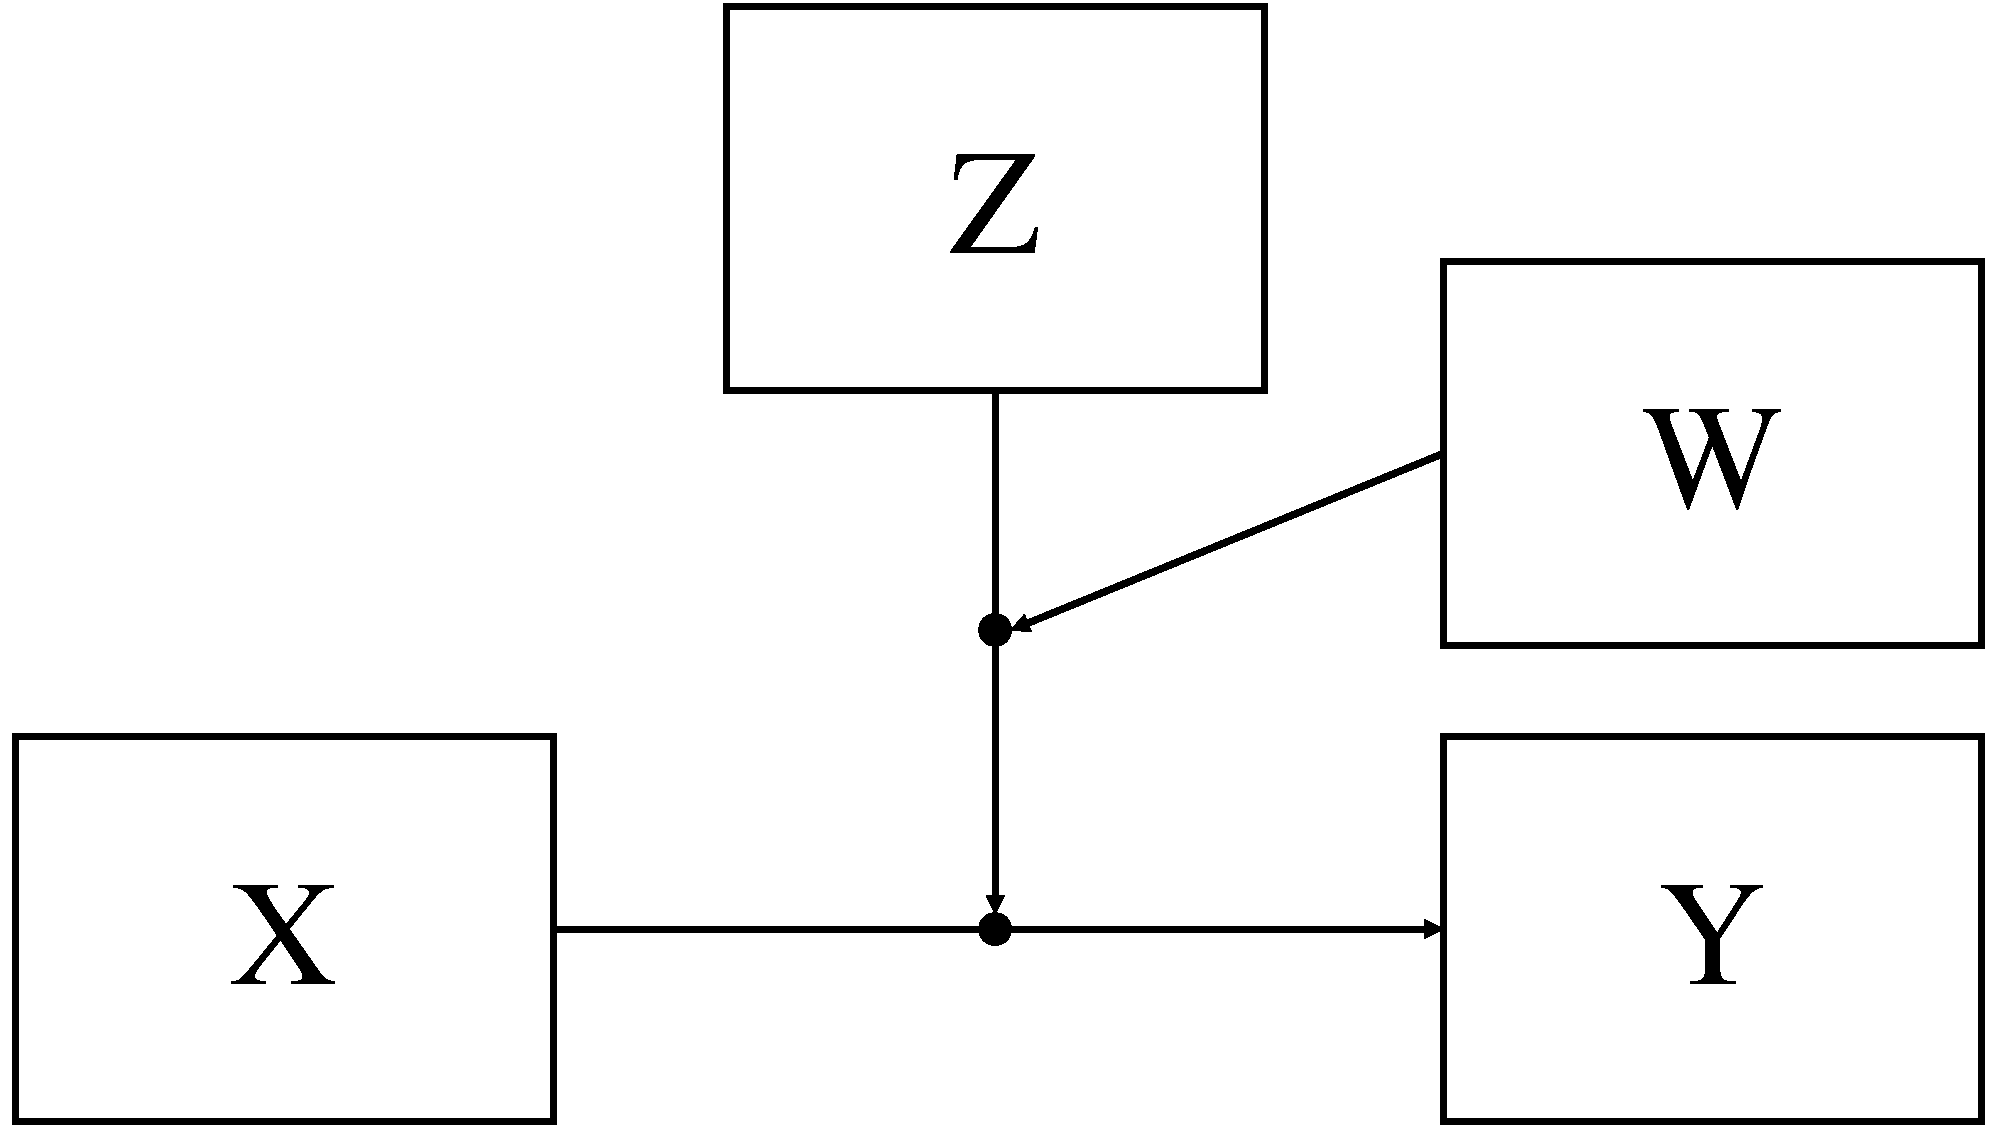
\includegraphics[width=\textwidth]{figures/threeWayConceptual.pdf}
  \end{figure}
  
\end{frame}



\begin{frame}{Moderated Moderation}
  
  The preceding conceptual diagram implies this analytic diagram:
  \begin{figure}
    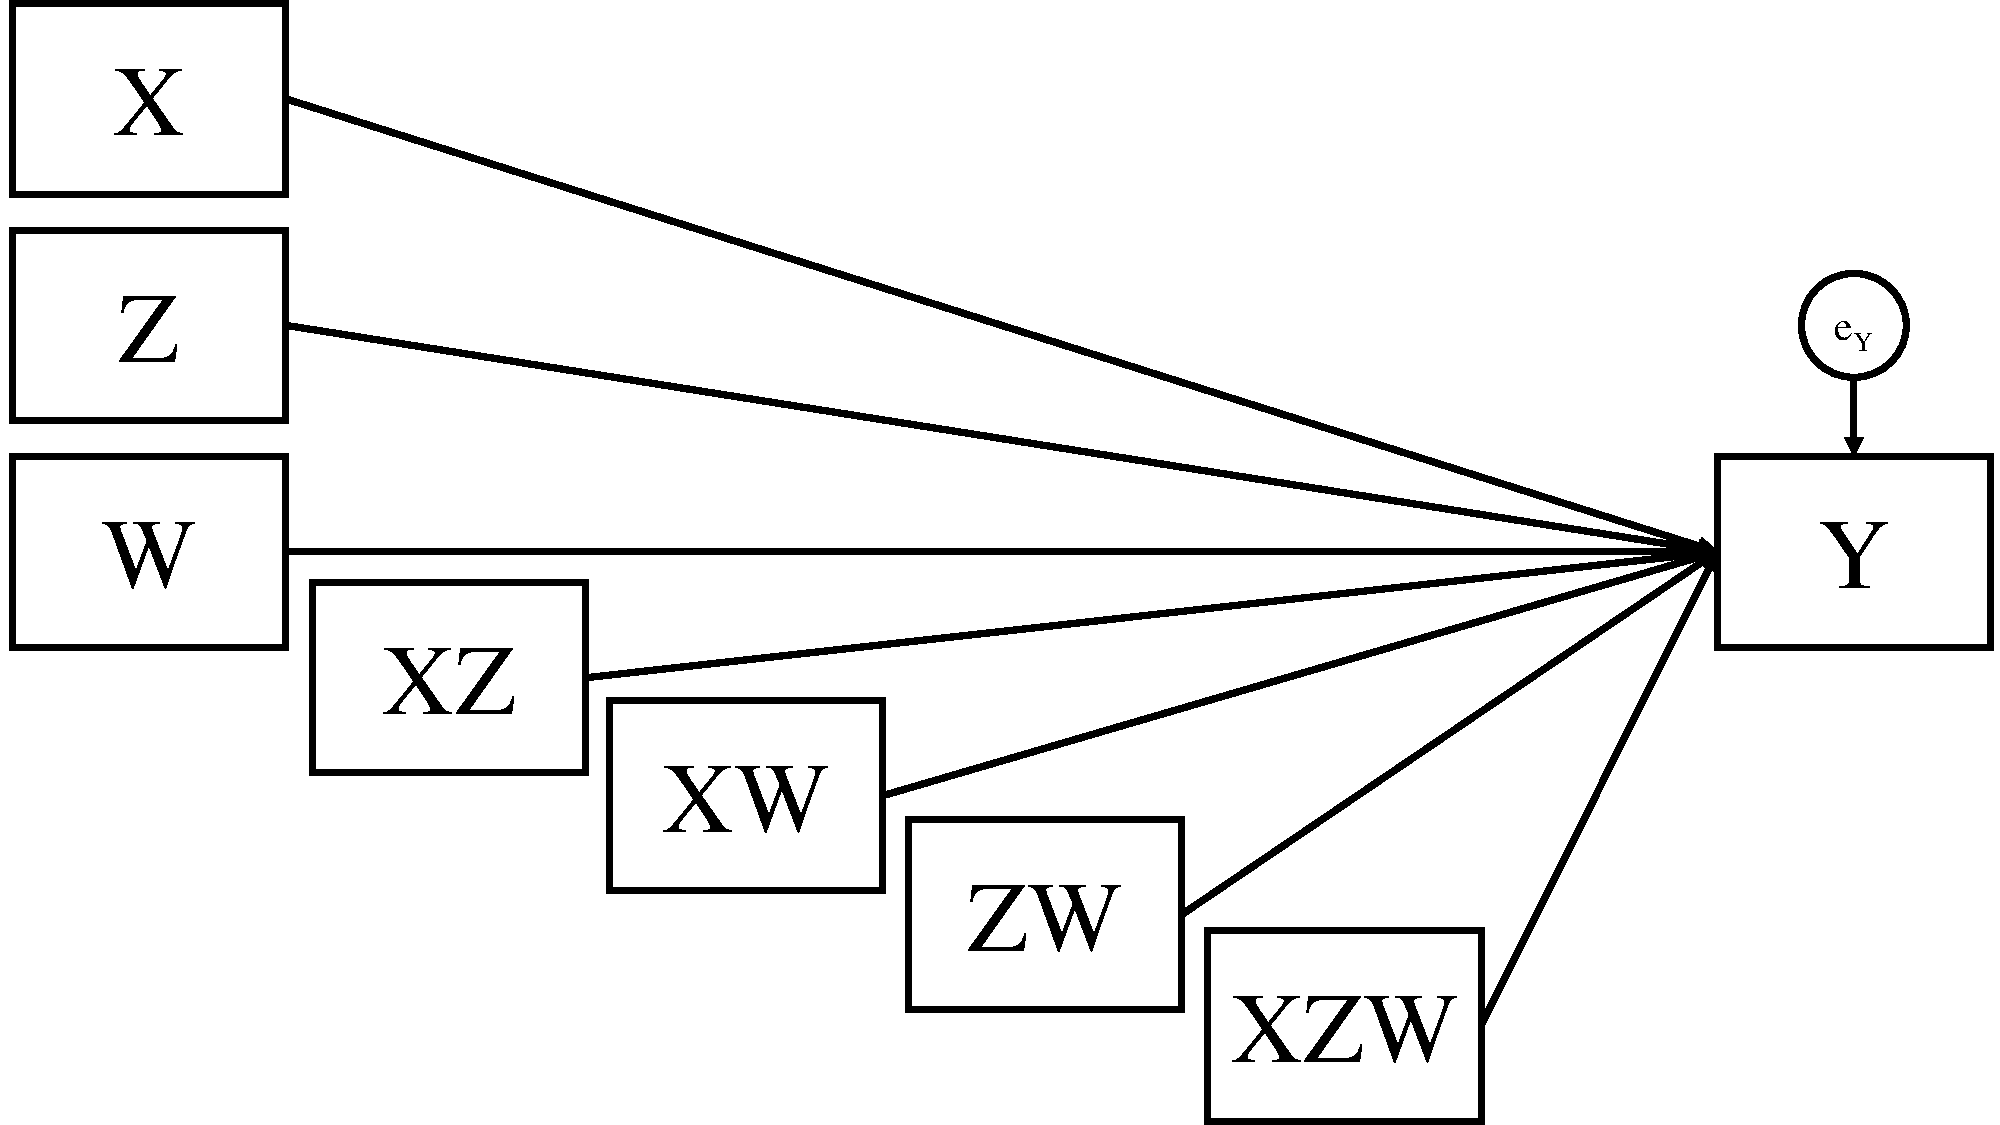
\includegraphics[width=\textwidth]{figures/threeWayAnalytic.pdf}
  \end{figure}
  
\end{frame}



\begin{frame}[shrink = 5]{Moderated Moderation}
  
  The preceding diagram represents the following equation:
  \begin{align*}
    Y =& ~ \alpha + \beta_1X + \beta_2Z + \beta_3W +\\
    &\beta_4XZ + \beta_5XW + \beta_6ZW + \beta_7XZW + e
  \end{align*}\\
  \vb
  Which can be restructured into:
  \begin{align*}
    Y =& ~ \alpha + (\beta_1 + \beta_4Z + \beta_5W + \beta_7ZW)X + \\
    &\beta_2Z + \beta_3W + \beta_6ZW + e\\
    =& ~ \alpha + g(Z, W)X + \beta_2Z + \beta_3W + \beta_6ZW + e
  \end{align*}\\
  \vb 
  With moderated moderation, the simple slope is given by:
  \begin{align*}
    g(Z, W) = \beta_1 + \beta_4Z + \beta_5W + \beta_7ZW
  \end{align*}\\
  \vb 
  Which has the same structure as a single moderator model.
  \vc
  \begin{itemize}
  \item Three-way simple slopes represent the moderated effect of
    $Z$ on the $X \rightarrow Y$ relation at conditional values of $W$.
  \end{itemize}
  
\end{frame}



\begin{frame}[allowframebreaks]{Example}
    
\begin{Schunk}
\begin{Sinput}
 ## Three-way interaction model:
 out1.3 <- lm(agree ~ open*conc*neuro, data = dat1)
 summary(out1.3)
\end{Sinput}
\begin{Soutput}
Call:
lm(formula = agree ~ open * conc * neuro, data = dat1)

Residuals:
     Min       1Q   Median       3Q      Max 
-2.79789 -0.41779  0.09925  0.47556  2.10928 

Coefficients:
                Estimate Std. Error t value Pr(>|t|)    
(Intercept)     -0.58747    0.96633  -0.608  0.54328    
open             1.27903    0.25747   4.968 7.23e-07 ***
conc             1.20831    0.26559   4.550 5.63e-06 ***
neuro            0.73766    0.32240   2.288  0.02222 *  
open:conc       -0.29722    0.06935  -4.286 1.89e-05 ***
open:neuro      -0.21616    0.08091  -2.672  0.00760 ** 
conc:neuro      -0.25632    0.08244  -3.109  0.00190 ** 
open:conc:neuro  0.06541    0.02028   3.225  0.00128 ** 
---
Signif. codes:  0 ‘***’ 0.001 ‘**’ 0.01 ‘*’ 0.05 ‘.’ 0.1 ‘ ’ 1

Residual standard error: 0.6945 on 2544 degrees of freedom
Multiple R-squared:  0.07189,	Adjusted R-squared:  0.06933 
F-statistic: 28.15 on 7 and 2544 DF,  p-value: < 2.2e-16
\end{Soutput}
\end{Schunk}


\pagebreak

\begin{Schunk}
\begin{Sinput}
 ## Test Differences between Indirect Effects
 ## in Serial Multiple Mediator Model (Method 1):
 mod2.3 <- "
 policy ~ cp*polAffil + b1*merit + b2*sysRac
 merit ~ a1*polAffil
 sysRac ~ a2*polAffil + d21*merit
 
 ab1 := a1*b1
 ab2 := a2*b2
 fullIE := a1*d21*b2
 totalIE := ab1 + ab2 + fullIE 
 
 fullIE == ab1
 fullIE == ab2
 "
 out2.3 <- 
     sem(mod2.3, data = dat1, se = "boot", boot = nBoot)
 summary(out2.3)
\end{Sinput}
\begin{Soutput}
lavaan (0.5-20) converged normally after 213 iterations

  Number of observations                            87

  Estimator                                         ML
  Minimum Function Test Statistic                1.334
  Degrees of freedom                                 2
  P-value (Chi-square)                           0.513

Parameter Estimates:

  Information                                 Observed
  Standard Errors                            Bootstrap
  Number of requested bootstrap draws             2500
  Number of successful bootstrap draws            2500

Regressions:
                   Estimate  Std.Err  Z-value  P(>|z|)
  policy ~                                            
    polAffil  (cp)    0.108    0.084    1.281    0.200
    merit     (b1)   -0.150    0.047   -3.183    0.001
    sysRac    (b2)    0.521    0.125    4.157    0.000
  merit ~                                             
    polAffil  (a1)   -0.271    0.057   -4.750    0.000
  sysRac ~                                            
    polAffil  (a2)    0.078    0.025    3.125    0.002
    merit    (d21)   -0.287    0.075   -3.814    0.000

Variances:
                   Estimate  Std.Err  Z-value  P(>|z|)
    policy            1.001    0.171    5.854    0.000
    merit             0.719    0.114    6.330    0.000
    sysRac            0.690    0.090    7.632    0.000

Defined Parameters:
                   Estimate  Std.Err  Z-value  P(>|z|)
    ab1               0.041    0.014    2.983    0.003
    ab2               0.041    0.014    2.983    0.003
    fullIE            0.041    0.014    2.983    0.003
    totalIE           0.122    0.041    2.983    0.003

Constraints:
                                               |Slack|
    fullIE - (ab1)                               0.000
    fullIE - (ab2)                               0.000
\end{Soutput}
\begin{Sinput}
 ## Conduct a chi-squared difference test:
 chiDiff <- fitMeasures(out2.3)["chisq"] - 
     fitMeasures(out2.1)["chisq"]
 dfDiff <- fitMeasures(out2.3)["df"] - 
     fitMeasures(out2.1)["df"]
 pchisq(chiDiff, dfDiff, lower = FALSE)
\end{Sinput}
\begin{Soutput}
    chisq 
0.5131246 
\end{Soutput}
\end{Schunk}


\pagebreak

\begin{Schunk}
\begin{Sinput}
 ## Conditional process model with b, c paths moderated:
 mod5 <- "
 agree ~ b1*open + b2*consc + cp1*extra + cp2*neuro + 
         cp3*extraXneuro + b3*openXconsc
 open ~ a*extra
 
 cpLo  := cp1 + cp3*(-0.962268)
 cpMid := cp1 + cp3*(-0.162268)
 cpHi  := cp1 + cp3*0.837732
 
 abLo := a * (b1 + b3*(-0.4045))
 abMid := a * (b1 + b3*(-0.0045))
 abHi := a * (b1 + b3*0.3955)
 "
\end{Sinput}
\end{Schunk}


\pagebreak

\begin{Schunk}
\begin{Sinput}
 out5 <- sem(mod5, data = dat1, se = "boot", boot = nBoot)
 summary(out5)
\end{Sinput}
\begin{Soutput}
lavaan (0.5-20) converged normally after  18 iterations

  Number of observations                          2800

  Estimator                                         ML
  Minimum Function Test Statistic              201.443
  Degrees of freedom                                 4
  P-value (Chi-square)                           0.000

Parameter Estimates:

  Information                                 Observed
  Standard Errors                            Bootstrap
  Number of requested bootstrap draws             5000
  Number of successful bootstrap draws            5000

Regressions:
                   Estimate  Std.Err  Z-value  P(>|z|)
  agree ~                                             
    open      (b1)    0.191    0.028    6.941    0.000
    consc     (b2)    0.021    0.027    0.774    0.439
    extra    (cp1)    0.349    0.027   13.030    0.000
    neuro    (cp2)   -0.102    0.012   -8.564    0.000
    extraXnr (cp3)    0.049    0.022    2.210    0.027
    opnXcnsc  (b3)   -0.074    0.044   -1.671    0.095
  open ~                                              
    extra      (a)    0.268    0.023   11.662    0.000

Variances:
                   Estimate  Std.Err  Z-value  P(>|z|)
    agree             0.471    0.014   32.521    0.000
    open              0.294    0.010   29.875    0.000

Defined Parameters:
                   Estimate  Std.Err  Z-value  P(>|z|)
    cpLo              0.302    0.036    8.459    0.000
    cpMid             0.341    0.027   12.473    0.000
    cpHi              0.390    0.031   12.502    0.000
    abLo              0.059    0.011    5.320    0.000
    abMid             0.051    0.009    5.778    0.000
    abHi              0.043    0.009    4.788    0.000
\end{Soutput}
\end{Schunk}


\pagebreak

\begin{Schunk}
\begin{Sinput}
 ## Hybrid Multiple Mediator Model:
 mod4.1 <- "
 policy ~ b1*merit + b21*sysRac + b22*revDisc + cp*polAffil
 sysRac ~ d211*merit + a21*polAffil
 revDisc ~ d221*merit + a22*polAffil
 merit ~ a1*polAffil
 
 sysRac ~~ revDisc
 
 ab1 := a1*b1
 ab21 := a21*b21
 ab22 := a22*b22
 
 fullIE21 := a1*d211*b21
 fullIE22 := a1*d221*b22
 
 totalIE := ab1 + ab21 + ab22 + fullIE21 + fullIE22
 "
 out4.1 <- 
     sem(mod4.1, data = dat1, se = "boot", boot = nBoot)
 summary(out4.1)
\end{Sinput}
\begin{Soutput}
lavaan (0.5-20) converged normally after  22 iterations

  Number of observations                            87

  Estimator                                         ML
  Minimum Function Test Statistic                0.000
  Degrees of freedom                                 0
  Minimum Function Value               0.0000000000000

Parameter Estimates:

  Information                                 Observed
  Standard Errors                            Bootstrap
  Number of requested bootstrap draws             2500
  Number of successful bootstrap draws            2499

Regressions:
                   Estimate  Std.Err  Z-value  P(>|z|)
  policy ~                                            
    merit     (b1)    0.005    0.142    0.035    0.972
    sysRac   (b21)    0.589    0.150    3.924    0.000
    revDisc  (b22)   -0.026    0.080   -0.328    0.743
    polAffl   (cp)    0.130    0.080    1.627    0.104
  sysRac ~                                            
    merit   (d211)   -0.301    0.111   -2.721    0.006
    polAffl  (a21)    0.090    0.070    1.282    0.200
  revDisc ~                                           
    merit   (d221)    0.532    0.192    2.777    0.005
    polAffl  (a22)   -0.167    0.138   -1.214    0.225
  merit ~                                             
    polAffl   (a1)   -0.266    0.061   -4.337    0.000

Covariances:
                   Estimate  Std.Err  Z-value  P(>|z|)
  sysRac ~~                                           
    revDisc          -0.135    0.157   -0.859    0.390

Variances:
                   Estimate  Std.Err  Z-value  P(>|z|)
    policy            0.985    0.162    6.098    0.000
    sysRac            0.689    0.092    7.463    0.000
    revDisc           2.388    0.303    7.881    0.000
    merit             0.719    0.113    6.378    0.000

Defined Parameters:
                   Estimate  Std.Err  Z-value  P(>|z|)
    ab1              -0.001    0.039   -0.034    0.973
    ab21              0.053    0.043    1.247    0.212
    ab22              0.004    0.018    0.251    0.801
    fullIE21          0.047    0.025    1.871    0.061
    fullIE22          0.004    0.014    0.276    0.783
    totalIE           0.107    0.052    2.047    0.041
\end{Soutput}
\end{Schunk}


\pagebreak

\begin{Schunk}
\begin{Sinput}
 parameterEstimates(out4.1, boot = bootType)[ , -c(1 : 3)]
\end{Sinput}
\begin{Soutput}
      label    est    se      z pvalue ci.lower ci.upper
1        b1  0.005 0.142  0.035  0.972   -0.266    0.285
2       b21  0.589 0.150  3.924  0.000    0.301    0.891
3       b22 -0.026 0.080 -0.328  0.743   -0.186    0.129
4        cp  0.130 0.080  1.627  0.104   -0.029    0.283
5      d211 -0.301 0.111 -2.721  0.006   -0.520   -0.085
6       a21  0.090 0.070  1.282  0.200   -0.045    0.222
7      d221  0.532 0.192  2.777  0.005    0.137    0.899
8       a22 -0.167 0.138 -1.214  0.225   -0.447    0.099
9        a1 -0.266 0.061 -4.337  0.000   -0.396   -0.153
10          -0.135 0.157 -0.859  0.390   -0.459    0.165
11           0.985 0.162  6.098  0.000    0.750    1.477
12           0.689 0.092  7.463  0.000    0.538    0.904
13           2.388 0.303  7.881  0.000    1.894    3.158
14           0.719 0.113  6.378  0.000    0.535    1.003
15           2.444 0.000     NA     NA    2.444    2.444
16      ab1 -0.001 0.039 -0.034  0.973   -0.081    0.074
17     ab21  0.053 0.043  1.247  0.212   -0.019    0.151
18     ab22  0.004 0.018  0.251  0.801   -0.018    0.064
19 fullIE21  0.047 0.025  1.871  0.061    0.013    0.123
20 fullIE22  0.004 0.014  0.276  0.783   -0.015    0.042
21  totalIE  0.107 0.052  2.047  0.041    0.005    0.218
\end{Soutput}
\end{Schunk}


\pagebreak

\begin{Schunk}
\begin{Sinput}
 ## Use semTools to orthogonalize:
 dat2.2 <- indProd(data = dat1,
                   var1 = c("x1", "x2", "x3"),
                   var2 = c("z1", "z2", "z3"),
                   match = FALSE,
                   residualC = TRUE)
 sum(dat2 - dat2.2)
\end{Sinput}
\begin{Soutput}
[1] -9.790839e-14
\end{Soutput}
\begin{Sinput}
 ##
 ## Use semTools to double mean center:
 dat3.2 <- indProd(data = dat1,
                   var1 = c("x1", "x2", "x3"),
                   var2 = c("z1", "z2", "z3"),
                   match = FALSE,
                   doubleMC = TRUE)
 sum(dat3[ , -c(1 : 9)] - dat3.2[ , -c(1 : 9)])
\end{Sinput}
\begin{Soutput}
[1] 0
\end{Soutput}
\end{Schunk}


\end{frame}



\begin{frame}[allowframebreaks]{Example}
  
\begin{Schunk}
\begin{Sinput}
 par(family = "serif", cex = 0.75)
 plotOut1.5 <- plotSlopes(model = out1.5,
                          plotx = "openXconc",
                          modx = "neuro",
                          plotPoints = FALSE,
                          modxVals = 
                          quantile(dat1$neuro,
                                   c(0.25, 0.5, 0.75),
                                   na.rm = TRUE)
                          )
\end{Sinput}
\end{Schunk}

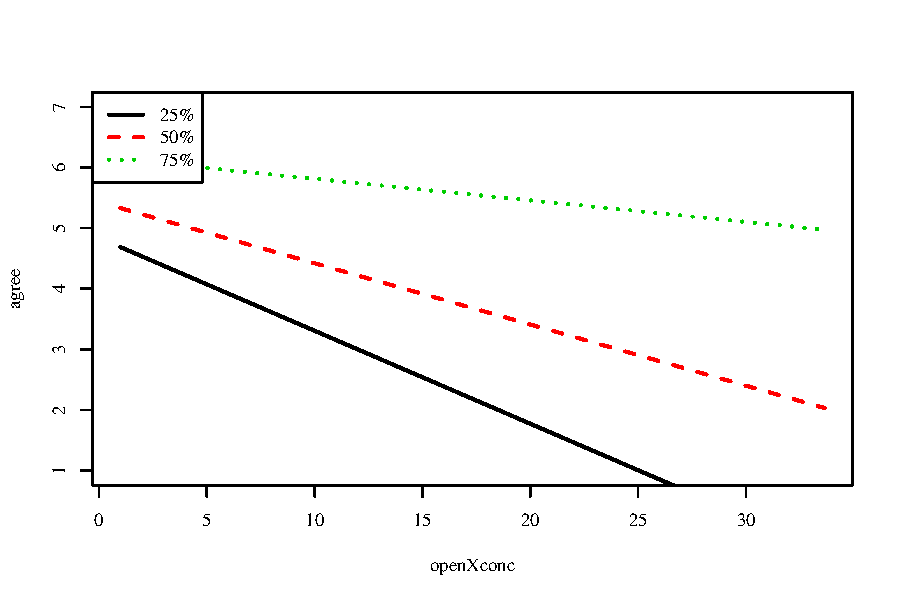
\includegraphics{sweaveFiles/-017}

\pagebreak

\begin{Schunk}
\begin{Sinput}
 par(family = "serif", cex = 0.75)
 testOut1.5 <- testSlopes(plotOut1.5)
\end{Sinput}
\begin{Soutput}
Values of neuro OUTSIDE this interval:
      lo       hi 
3.343832 7.745048 
cause the slope of (b1 + b2*neuro)openXconc to be statistically significant
\end{Soutput}
\begin{Sinput}
 plot(testOut1.5)
\end{Sinput}
\end{Schunk}

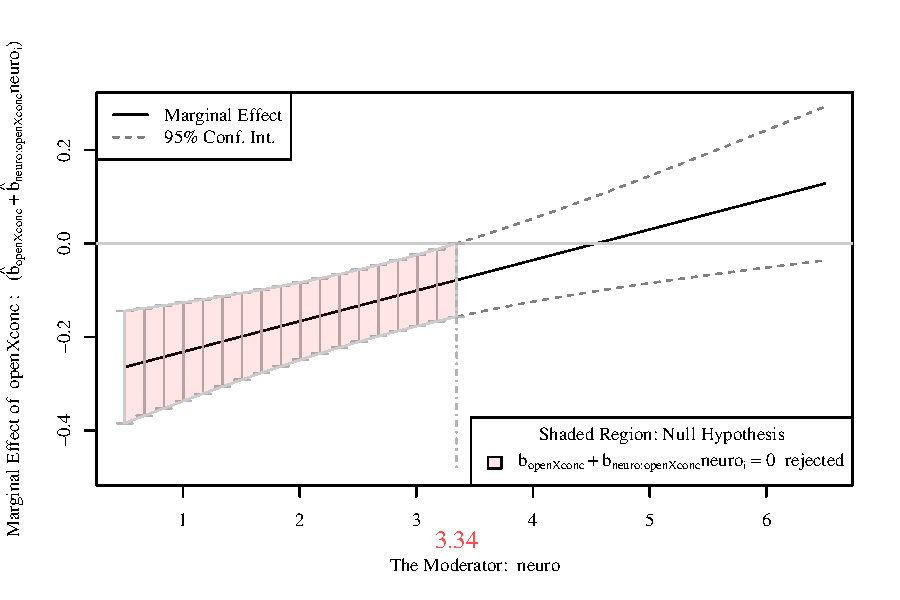
\includegraphics{sweaveFiles/-018}

\end{frame}



\begin{frame}{Categorical Variable Moderation}
  
  When the moderator is a categorical variable, moderation implies
  between-group differences in the focal effect.  
  \va
  \begin{itemize}
    \item This simplifies probing considerably
      \vb
    \item The simple slopes are given (almost) directly in the output
  \end{itemize}
  \va
  Recall the simple slope formula:
  \begin{align*}
    SS = \beta_1 + \beta_3Z
  \end{align*}
  Because $Z$ is a dummy code, this formula reduces to:
  \begin{align*}
    SS &= \beta_1, \text{ or}\\
    SS &= \beta_1 + \beta_3
  \end{align*}

\end{frame}



\begin{frame}[allowframebreaks]{Example}

\begin{Schunk}
\begin{Sinput}
 ## Marginal focal effect:
 out2.1 <- lm(conc ~ neuro, data = dat1)
 summary(out2.1)
\end{Sinput}
\begin{Soutput}
Call:
lm(formula = conc ~ neuro, data = dat1)

Residuals:
     Min       1Q   Median       3Q      Max 
-2.55547 -0.33353  0.00824  0.36098  1.85381 

Coefficients:
            Estimate Std. Error t value Pr(>|t|)    
(Intercept) 3.437327   0.029659  115.90   <2e-16 ***
neuro       0.118144   0.008844   13.36   <2e-16 ***
---
Signif. codes:  0 ‘***’ 0.001 ‘**’ 0.01 ‘*’ 0.05 ‘.’ 0.1 ‘ ’ 1

Residual standard error: 0.533 on 2550 degrees of freedom
Multiple R-squared:  0.0654,	Adjusted R-squared:  0.06504 
F-statistic: 178.4 on 1 and 2550 DF,  p-value: < 2.2e-16
\end{Soutput}
\begin{Sinput}
 ## Moderated by highest education attained:
 out2.2 <- lm(conc ~ neuro*educ, data = dat1)
 summary(out2.2)
\end{Sinput}
\begin{Soutput}
Call:
lm(formula = conc ~ neuro * educ, data = dat1)

Residuals:
     Min       1Q   Median       3Q      Max 
-2.52324 -0.34119  0.01457  0.36247  1.86213 

Coefficients:
            Estimate Std. Error t value Pr(>|t|)    
(Intercept)  3.72924    0.10864  34.326  < 2e-16 ***
neuro        0.01259    0.03156   0.399 0.689990    
educ2       -0.32892    0.11497  -2.861 0.004258 ** 
educ3       -0.30738    0.12102  -2.540 0.011146 *  
neuro:educ2  0.11033    0.03346   3.297 0.000990 ***
neuro:educ3  0.12755    0.03552   3.591 0.000336 ***
---
Signif. codes:  0 ‘***’ 0.001 ‘**’ 0.01 ‘*’ 0.05 ‘.’ 0.1 ‘ ’ 1

Residual standard error: 0.5308 on 2546 degrees of freedom
Multiple R-squared:  0.0746,	Adjusted R-squared:  0.07278 
F-statistic: 41.05 on 5 and 2546 DF,  p-value: < 2.2e-16
\end{Soutput}
\begin{Sinput}
 ## Test for omnibus moderation:
 anova(out2.1, out2.2)
\end{Sinput}
\begin{Soutput}
Analysis of Variance Table

Model 1: conc ~ neuro
Model 2: conc ~ neuro * educ
  Res.Df    RSS Df Sum of Sq      F    Pr(>F)    
1   2550 724.47                                  
2   2546 717.35  4    7.1285 6.3251 4.617e-05 ***
---
Signif. codes:  0 ‘***’ 0.001 ‘**’ 0.01 ‘*’ 0.05 ‘.’ 0.1 ‘ ’ 1
\end{Soutput}
\end{Schunk}


\pagebreak

\begin{Schunk}
\begin{Sinput}
 par(family = "serif", cex = 0.75)
 plotSlopes(out2.2,
            plotx = "neuro",
            modx = "educ",
            plotPoints = FALSE)
\end{Sinput}
\end{Schunk}

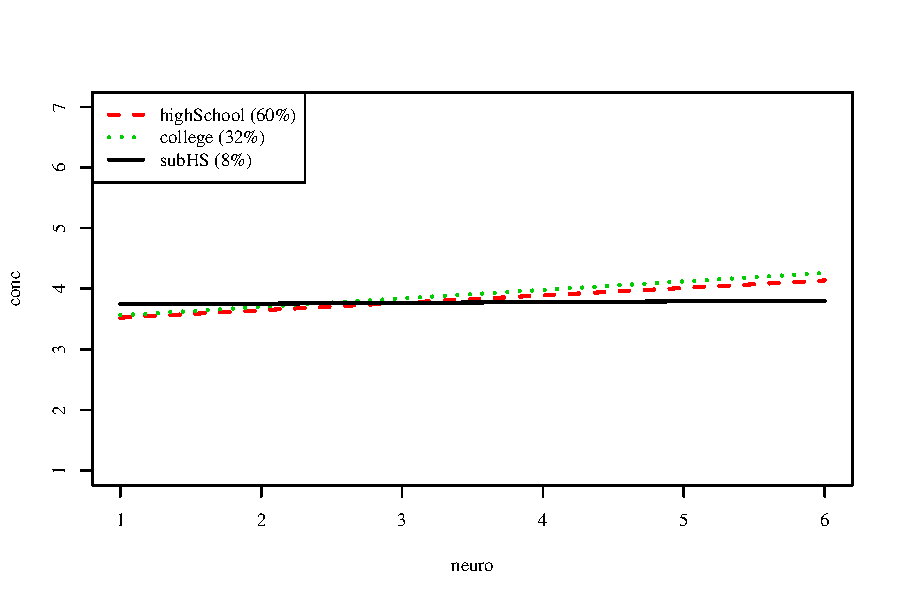
\includegraphics{sweaveFiles/-020}

\pagebreak

\begin{Schunk}
\begin{Sinput}
 ## Compute simple slopes by hand:
 ssSubHS <- coef(out2.2)[2]
 ssHighSchool <- sum(coef(out2.2)[c(2, 5)])
 ssCollege <- sum(coef(out2.2)[c(2, 6)])
 ## Compute simple slopes using centering:
 dat1$educ2 <- relevel(dat1$educ, ref = "highSchool")
 dat1$educ3 <- relevel(dat1$educ, ref = "college")
 out2.3 <- lm(conc ~ neuro*educ2, data = dat1)
 out2.4 <- lm(conc ~ neuro*educ3, data = dat1)
\end{Sinput}
\end{Schunk}


\pagebreak

\begin{Schunk}
\begin{Sinput}
 ## By hand:
 ssSubHS
\end{Sinput}
\begin{Soutput}
    neuro 
0.0125915 
\end{Soutput}
\begin{Sinput}
 ## By centering:
 as.matrix(coef(out2.2))
\end{Sinput}
\begin{Soutput}
                  [,1]
(Intercept)  3.7292366
neuro        0.0125915
educ2       -0.3289176
educ3       -0.3073786
neuro:educ2  0.1103337
neuro:educ3  0.1275497
\end{Soutput}
\end{Schunk}


\pagebreak

\begin{Schunk}
\begin{Sinput}
 ## By hand:
 ssHighSchool
\end{Sinput}
\begin{Soutput}
[1] 0.1229252
\end{Soutput}
\begin{Sinput}
 ## By centering:
 as.matrix(coef(out2.3))
\end{Sinput}
\begin{Soutput}
                          [,1]
(Intercept)         3.40031894
neuro               0.12292519
educ2subHS          0.32891761
educ2college        0.02153898
neuro:educ2subHS   -0.11033369
neuro:educ2college  0.01721601
\end{Soutput}
\end{Schunk}


\pagebreak

\begin{Schunk}
\begin{Sinput}
 ## By hand:
 ssCollege
\end{Sinput}
\begin{Soutput}
[1] 0.1401412
\end{Soutput}
\begin{Sinput}
 ## By centering:
 as.matrix(coef(out2.4))
\end{Sinput}
\begin{Soutput}
                             [,1]
(Intercept)            3.42185792
neuro                  0.14014120
educ3subHS             0.30737863
educ3highSchool       -0.02153898
neuro:educ3subHS      -0.12754971
neuro:educ3highSchool -0.01721601
\end{Soutput}
\end{Schunk}


\end{frame}



\begin{frame}[shrink = 10]{Example}

\begin{Schunk}
\begin{Sinput}
 summary(out2.2)
\end{Sinput}
\begin{Soutput}
Call:
lm(formula = conc ~ neuro * educ, data = dat1)

Residuals:
     Min       1Q   Median       3Q      Max 
-2.52324 -0.34119  0.01457  0.36247  1.86213 

Coefficients:
            Estimate Std. Error t value Pr(>|t|)    
(Intercept)  3.72924    0.10864  34.326  < 2e-16 ***
neuro        0.01259    0.03156   0.399 0.689990    
educ2       -0.32892    0.11497  -2.861 0.004258 ** 
educ3       -0.30738    0.12102  -2.540 0.011146 *  
neuro:educ2  0.11033    0.03346   3.297 0.000990 ***
neuro:educ3  0.12755    0.03552   3.591 0.000336 ***
---
Signif. codes:  0 ‘***’ 0.001 ‘**’ 0.01 ‘*’ 0.05 ‘.’ 0.1 ‘ ’ 1

Residual standard error: 0.5308 on 2546 degrees of freedom
Multiple R-squared:  0.0746,	Adjusted R-squared:  0.07278 
F-statistic: 41.05 on 5 and 2546 DF,  p-value: < 2.2e-16
\end{Soutput}
\end{Schunk}


\end{frame}



\begin{frame}[shrink = 10]{Example}

\begin{Schunk}
\begin{Sinput}
 summary(out2.3)
\end{Sinput}
\begin{Soutput}
Call:
lm(formula = conc ~ neuro * educ2, data = dat1)

Residuals:
     Min       1Q   Median       3Q      Max 
-2.52324 -0.34119  0.01457  0.36247  1.86213 

Coefficients:
                   Estimate Std. Error t value Pr(>|t|)    
(Intercept)         3.40032    0.03761  90.401  < 2e-16 ***
neuro               0.12293    0.01111  11.063  < 2e-16 ***
educ2subHS          0.32892    0.11497   2.861  0.00426 ** 
educ2college        0.02154    0.06525   0.330  0.74134    
neuro:educ2subHS   -0.11033    0.03346  -3.297  0.00099 ***
neuro:educ2college  0.01722    0.01972   0.873  0.38277    
---
Signif. codes:  0 ‘***’ 0.001 ‘**’ 0.01 ‘*’ 0.05 ‘.’ 0.1 ‘ ’ 1

Residual standard error: 0.5308 on 2546 degrees of freedom
Multiple R-squared:  0.0746,	Adjusted R-squared:  0.07278 
F-statistic: 41.05 on 5 and 2546 DF,  p-value: < 2.2e-16
\end{Soutput}
\end{Schunk}


\end{frame}



\begin{frame}[shrink = 10]{Example}

\begin{Schunk}
\begin{Sinput}
 summary(out2.4)
\end{Sinput}
\begin{Soutput}
Call:
lm(formula = conc ~ neuro * educ3, data = dat1)

Residuals:
     Min       1Q   Median       3Q      Max 
-2.52324 -0.34119  0.01457  0.36247  1.86213 

Coefficients:
                      Estimate Std. Error t value Pr(>|t|)    
(Intercept)            3.42186    0.05331  64.183  < 2e-16 ***
neuro                  0.14014    0.01629   8.601  < 2e-16 ***
educ3subHS             0.30738    0.12102   2.540 0.011146 *  
educ3highSchool       -0.02154    0.06525  -0.330 0.741340    
neuro:educ3subHS      -0.12755    0.03552  -3.591 0.000336 ***
neuro:educ3highSchool -0.01722    0.01972  -0.873 0.382770    
---
Signif. codes:  0 ‘***’ 0.001 ‘**’ 0.01 ‘*’ 0.05 ‘.’ 0.1 ‘ ’ 1

Residual standard error: 0.5308 on 2546 degrees of freedom
Multiple R-squared:  0.0746,	Adjusted R-squared:  0.07278 
F-statistic: 41.05 on 5 and 2546 DF,  p-value: < 2.2e-16
\end{Soutput}
\end{Schunk}


\end{frame}




\begin{frame}{Moderation via Multiple Group SEM}
  
  When our moderator is a categorical variable, we can use multiple
  group CFA/SEM to test for moderation.
  \va
  \begin{itemize}
    \item Categorical moderators define groups
      \vb
    \item Significant moderation with categorical moderators implies
      between-group differences in the focal effect
      \vb
    \item These hypotheses are easily tested with multiple group SEM
  \end{itemize}
  \va
  \begin{center}\textsc{Whiteboard Time!}\end{center}
  
\end{frame}



\begin{frame}[allowframebreaks]{Example}

\begin{Schunk}
\begin{Sinput}
 library(lavaan)
 library(semTools)
 dat2 <- readRDS("../data/bfiData2.rds")
 ## Multiple group moderation:
 mod1 <- "
 conc =~ C1 + C2 + C3 + C4 + C5
 neuro =~ N1 + N2 + N3 + N4 + N5
 "
\end{Sinput}
\end{Schunk}


\end{frame}



\begin{frame}[shrink = 10]{Example}
  
\begin{Schunk}
\begin{Sinput}
 fit1 <- measurementInvariance(mod1,
                               data = dat2,
                               group = "educ",
                               std.lv = TRUE)
\end{Sinput}
\begin{Soutput}
Measurement invariance models:

Model 1 : fit.configural
Model 2 : fit.loadings
Model 3 : fit.intercepts
Model 4 : fit.means

Chi Square Difference Test

                Df   AIC   BIC  Chisq Chisq diff Df diff Pr(>Chisq)    
fit.configural 102 85428 85971 1039.1                                  
fit.loadings   118 85427 85877 1070.0     30.927      16  0.0137462 *  
fit.intercepts 134 85456 85813 1131.4     61.399      16  3.037e-07 ***
fit.means      138 85468 85801 1150.8     19.324       4  0.0006788 ***
---
Signif. codes:  0 ‘***’ 0.001 ‘**’ 0.01 ‘*’ 0.05 ‘.’ 0.1 ‘ ’ 1


Fit measures:

                 cfi rmsea cfi.delta rmsea.delta
fit.configural 0.874 0.104        NA          NA
fit.loadings   0.871 0.097     0.002       0.007
fit.intercepts 0.865 0.094     0.006       0.004
fit.means      0.863 0.093     0.002       0.001
\end{Soutput}
\end{Schunk}


\end{frame}


\begin{frame}[allowframebreaks]{Example}

\begin{Schunk}
\begin{Sinput}
 mod2 <- "
 conc =~ C1 + C2 + C3 + C4 + C5
 neuro =~ N1 + N2 + N3 + N4 + N5
 
 conc ~ neuro
 
 conc ~~ c(1.0, NA, NA)*conc
 neuro ~~ c(1.0, NA, NA)*neuro
 
 conc ~ c(0.0, NA, NA)*1.0
 neuro ~ c(0.0, NA, NA)*1.0
 "
\end{Sinput}
\end{Schunk}


\pagebreak

\begin{Schunk}
\begin{Sinput}
 fit2 <- lavaan(mod2,
                data = dat2,
                std.lv = FALSE,
                auto.fix.first = FALSE,
                auto.var = TRUE,
                int.ov.free = TRUE,
                group = "educ",
                group.equal = c("loadings", "intercepts")
                )
\end{Sinput}
\end{Schunk}


\pagebreak

\begin{Schunk}
\begin{Sinput}
 summary(fit2)
\end{Sinput}
\begin{Soutput}
lavaan (0.5-20) converged normally after  79 iterations

  Number of observations per group         
  highSchool                                      1536
  subHS                                            192
  college                                          824

  Estimator                                         ML
  Minimum Function Test Statistic             1131.438
  Degrees of freedom                               134
  P-value (Chi-square)                           0.000

Chi-square for each group:

  highSchool                                   573.289
  subHS                                        108.925
  college                                      449.224

Parameter Estimates:

  Information                                 Expected
  Standard Errors                             Standard


Group 1 [highSchool]:

Latent Variables:
                   Estimate  Std.Err  Z-value  P(>|z|)
  conc =~                                             
    C1      (.p1.)    0.573    0.027   21.471    0.000
    C2      (.p2.)    0.678    0.029   23.706    0.000
    C3      (.p3.)    0.634    0.028   22.666    0.000
    C4      (.p4.)   -0.897    0.031  -29.235    0.000
    C5      (.p5.)   -0.947    0.036  -26.307    0.000
  neuro =~                                            
    N1      (.p6.)    1.305    0.033   39.285    0.000
    N2      (.p7.)    1.247    0.032   38.701    0.000
    N3      (.p8.)    1.205    0.034   35.309    0.000
    N4      (.p9.)    0.909    0.034   26.982    0.000
    N5      (.10.)    0.837    0.035   23.998    0.000

Regressions:
                   Estimate  Std.Err  Z-value  P(>|z|)
  conc ~                                              
    neuro            -0.359    0.035  -10.208    0.000

Intercepts:
                   Estimate  Std.Err  Z-value  P(>|z|)
    conc              0.000                           
    neuro             0.000                           
    C1      (.26.)    4.571    0.027  170.017    0.000
    C2      (.27.)    4.442    0.029  152.180    0.000
    C3      (.28.)    4.379    0.028  154.381    0.000
    C4      (.29.)    2.434    0.032   75.721    0.000
    C5      (.30.)    3.186    0.037   85.494    0.000
    N1      (.31.)    2.940    0.039   75.566    0.000
    N2      (.32.)    3.509    0.038   93.494    0.000
    N3      (.33.)    3.224    0.038   83.772    0.000
    N4      (.34.)    3.197    0.035   91.203    0.000
    N5      (.35.)    2.975    0.035   84.171    0.000

Variances:
                   Estimate  Std.Err  Z-value  P(>|z|)
    conc              1.000                           
    neuro             1.000                           
    C1                1.109    0.045   24.781    0.000
    C2                1.187    0.050   23.872    0.000
    C3                1.201    0.049   24.414    0.000
    C4                0.893    0.048   18.572    0.000
    C5                1.600    0.073   22.053    0.000
    N1                0.840    0.046   18.316    0.000
    N2                0.830    0.044   19.003    0.000
    N3                1.219    0.055   22.298    0.000
    N4                1.701    0.067   25.564    0.000
    N5                1.962    0.075   26.138    0.000


Group 2 [subHS]:

Latent Variables:
                   Estimate  Std.Err  Z-value  P(>|z|)
  conc =~                                             
    C1      (.p1.)    0.573    0.027   21.471    0.000
    C2      (.p2.)    0.678    0.029   23.706    0.000
    C3      (.p3.)    0.634    0.028   22.666    0.000
    C4      (.p4.)   -0.897    0.031  -29.235    0.000
    C5      (.p5.)   -0.947    0.036  -26.307    0.000
  neuro =~                                            
    N1      (.p6.)    1.305    0.033   39.285    0.000
    N2      (.p7.)    1.247    0.032   38.701    0.000
    N3      (.p8.)    1.205    0.034   35.309    0.000
    N4      (.p9.)    0.909    0.034   26.982    0.000
    N5      (.10.)    0.837    0.035   23.998    0.000

Regressions:
                   Estimate  Std.Err  Z-value  P(>|z|)
  conc ~                                              
    neuro            -0.252    0.105   -2.396    0.017

Intercepts:
                   Estimate  Std.Err  Z-value  P(>|z|)
    conc             -0.261    0.095   -2.741    0.006
    neuro             0.016    0.081    0.202    0.840
    C1      (.26.)    4.571    0.027  170.017    0.000
    C2      (.27.)    4.442    0.029  152.180    0.000
    C3      (.28.)    4.379    0.028  154.381    0.000
    C4      (.29.)    2.434    0.032   75.721    0.000
    C5      (.30.)    3.186    0.037   85.494    0.000
    N1      (.31.)    2.940    0.039   75.566    0.000
    N2      (.32.)    3.509    0.038   93.494    0.000
    N3      (.33.)    3.224    0.038   83.772    0.000
    N4      (.34.)    3.197    0.035   91.203    0.000
    N5      (.35.)    2.975    0.035   84.171    0.000

Variances:
                   Estimate  Std.Err  Z-value  P(>|z|)
    conc              1.061    0.170    6.237    0.000
    neuro             0.905    0.120    7.540    0.000
    C1                1.263    0.142    8.919    0.000
    C2                1.270    0.148    8.568    0.000
    C3                1.437    0.162    8.855    0.000
    C4                1.192    0.160    7.466    0.000
    C5                1.748    0.217    8.039    0.000
    N1                1.014    0.146    6.965    0.000
    N2                1.236    0.161    7.681    0.000
    N3                1.310    0.165    7.937    0.000
    N4                1.507    0.170    8.888    0.000
    N5                2.042    0.221    9.232    0.000


Group 3 [college]:

Latent Variables:
                   Estimate  Std.Err  Z-value  P(>|z|)
  conc =~                                             
    C1      (.p1.)    0.573    0.027   21.471    0.000
    C2      (.p2.)    0.678    0.029   23.706    0.000
    C3      (.p3.)    0.634    0.028   22.666    0.000
    C4      (.p4.)   -0.897    0.031  -29.235    0.000
    C5      (.p5.)   -0.947    0.036  -26.307    0.000
  neuro =~                                            
    N1      (.p6.)    1.305    0.033   39.285    0.000
    N2      (.p7.)    1.247    0.032   38.701    0.000
    N3      (.p8.)    1.205    0.034   35.309    0.000
    N4      (.p9.)    0.909    0.034   26.982    0.000
    N5      (.10.)    0.837    0.035   23.998    0.000

Regressions:
                   Estimate  Std.Err  Z-value  P(>|z|)
  conc ~                                              
    neuro            -0.278    0.052   -5.354    0.000

Intercepts:
                   Estimate  Std.Err  Z-value  P(>|z|)
    conc             -0.168    0.053   -3.139    0.002
    neuro            -0.092    0.045   -2.056    0.040
    C1      (.26.)    4.571    0.027  170.017    0.000
    C2      (.27.)    4.442    0.029  152.180    0.000
    C3      (.28.)    4.379    0.028  154.381    0.000
    C4      (.29.)    2.434    0.032   75.721    0.000
    C5      (.30.)    3.186    0.037   85.494    0.000
    N1      (.31.)    2.940    0.039   75.566    0.000
    N2      (.32.)    3.509    0.038   93.494    0.000
    N3      (.33.)    3.224    0.038   83.772    0.000
    N4      (.34.)    3.197    0.035   91.203    0.000
    N5      (.35.)    2.975    0.035   84.171    0.000

Variances:
                   Estimate  Std.Err  Z-value  P(>|z|)
    conc              1.139    0.098   11.634    0.000
    neuro             0.865    0.063   13.807    0.000
    C1                1.178    0.064   18.364    0.000
    C2                1.142    0.065   17.467    0.000
    C3                1.093    0.062   17.713    0.000
    C4                0.952    0.067   14.255    0.000
    C5                1.633    0.100   16.405    0.000
    N1                0.807    0.058   13.850    0.000
    N2                0.820    0.057   14.498    0.000
    N3                1.122    0.068   16.394    0.000
    N4                1.630    0.087   18.807    0.000
    N5                1.882    0.098   19.207    0.000
\end{Soutput}
\end{Schunk}


\pagebreak

\begin{Schunk}
\begin{Sinput}
 mod3 <- "
 conc =~ C1 + C2 + C3 + C4 + C5
 neuro =~ N1 + N2 + N3 + N4 + N5
 
 conc ~ c(b1, b1, b1)*neuro
 
 conc ~~ c(1.0, NA, NA)*conc
 neuro ~~ c(1.0, NA, NA)*neuro
 
 conc ~ c(0.0, NA, NA)*1.0
 neuro ~ c(0.0, NA, NA)*1.0
 "
\end{Sinput}
\end{Schunk}


\pagebreak

\begin{Schunk}
\begin{Sinput}
 fit3 <- lavaan(mod3,
                data = dat2,
                std.lv = FALSE,
                auto.fix.first = FALSE,
                auto.var = TRUE,
                int.ov.free = TRUE,
                group = "educ",
                group.equal = c("loadings", "intercepts")
                )
\end{Sinput}
\end{Schunk}


\pagebreak

\begin{Schunk}
\begin{Sinput}
 summary(fit3)
\end{Sinput}
\begin{Soutput}
lavaan (0.5-20) converged normally after  82 iterations

  Number of observations per group         
  highSchool                                      1536
  subHS                                            192
  college                                          824

  Estimator                                         ML
  Minimum Function Test Statistic             1133.785
  Degrees of freedom                               136
  P-value (Chi-square)                           0.000

Chi-square for each group:

  highSchool                                   574.222
  subHS                                        109.473
  college                                      450.090

Parameter Estimates:

  Information                                 Expected
  Standard Errors                             Standard


Group 1 [highSchool]:

Latent Variables:
                   Estimate  Std.Err  Z-value  P(>|z|)
  conc =~                                             
    C1      (.p1.)    0.575    0.027   21.516    0.000
    C2      (.p2.)    0.679    0.029   23.743    0.000
    C3      (.p3.)    0.635    0.028   22.707    0.000
    C4      (.p4.)   -0.898    0.031  -29.262    0.000
    C5      (.p5.)   -0.949    0.036  -26.367    0.000
  neuro =~                                            
    N1      (.p6.)    1.307    0.033   39.323    0.000
    N2      (.p7.)    1.249    0.032   38.734    0.000
    N3      (.p8.)    1.207    0.034   35.334    0.000
    N4      (.p9.)    0.910    0.034   26.987    0.000
    N5      (.10.)    0.839    0.035   24.010    0.000

Regressions:
                   Estimate  Std.Err  Z-value  P(>|z|)
  conc ~                                              
    neuro     (b1)   -0.330    0.029  -11.365    0.000

Intercepts:
                   Estimate  Std.Err  Z-value  P(>|z|)
    conc              0.000                           
    neuro             0.000                           
    C1      (.26.)    4.571    0.027  170.418    0.000
    C2      (.27.)    4.442    0.029  152.673    0.000
    C3      (.28.)    4.379    0.028  154.796    0.000
    C4      (.29.)    2.434    0.032   76.041    0.000
    C5      (.30.)    3.187    0.037   85.740    0.000
    N1      (.31.)    2.940    0.039   75.506    0.000
    N2      (.32.)    3.509    0.038   93.434    0.000
    N3      (.33.)    3.224    0.039   83.699    0.000
    N4      (.34.)    3.197    0.035   91.151    0.000
    N5      (.35.)    2.975    0.035   84.126    0.000

Variances:
                   Estimate  Std.Err  Z-value  P(>|z|)
    conc              1.000                           
    neuro             1.000                           
    C1                1.107    0.045   24.765    0.000
    C2                1.184    0.050   23.859    0.000
    C3                1.199    0.049   24.404    0.000
    C4                0.898    0.048   18.626    0.000
    C5                1.603    0.073   22.047    0.000
    N1                0.838    0.046   18.279    0.000
    N2                0.828    0.044   18.968    0.000
    N3                1.219    0.055   22.286    0.000
    N4                1.703    0.067   25.564    0.000
    N5                1.963    0.075   26.136    0.000


Group 2 [subHS]:

Latent Variables:
                   Estimate  Std.Err  Z-value  P(>|z|)
  conc =~                                             
    C1      (.p1.)    0.575    0.027   21.516    0.000
    C2      (.p2.)    0.679    0.029   23.743    0.000
    C3      (.p3.)    0.635    0.028   22.707    0.000
    C4      (.p4.)   -0.898    0.031  -29.262    0.000
    C5      (.p5.)   -0.949    0.036  -26.367    0.000
  neuro =~                                            
    N1      (.p6.)    1.307    0.033   39.323    0.000
    N2      (.p7.)    1.249    0.032   38.734    0.000
    N3      (.p8.)    1.207    0.034   35.334    0.000
    N4      (.p9.)    0.910    0.034   26.987    0.000
    N5      (.10.)    0.839    0.035   24.010    0.000

Regressions:
                   Estimate  Std.Err  Z-value  P(>|z|)
  conc ~                                              
    neuro     (b1)   -0.330    0.029  -11.365    0.000

Intercepts:
                   Estimate  Std.Err  Z-value  P(>|z|)
    conc             -0.259    0.095   -2.721    0.007
    neuro             0.016    0.081    0.201    0.841
    C1      (.26.)    4.571    0.027  170.418    0.000
    C2      (.27.)    4.442    0.029  152.673    0.000
    C3      (.28.)    4.379    0.028  154.796    0.000
    C4      (.29.)    2.434    0.032   76.041    0.000
    C5      (.30.)    3.187    0.037   85.740    0.000
    N1      (.31.)    2.940    0.039   75.506    0.000
    N2      (.32.)    3.509    0.038   93.434    0.000
    N3      (.33.)    3.224    0.039   83.699    0.000
    N4      (.34.)    3.197    0.035   91.151    0.000
    N5      (.35.)    2.975    0.035   84.126    0.000

Variances:
                   Estimate  Std.Err  Z-value  P(>|z|)
    conc              1.054    0.169    6.216    0.000
    neuro             0.896    0.119    7.551    0.000
    C1                1.264    0.142    8.917    0.000
    C2                1.272    0.148    8.569    0.000
    C3                1.434    0.162    8.851    0.000
    C4                1.196    0.160    7.477    0.000
    C5                1.742    0.217    8.026    0.000
    N1                1.013    0.145    6.978    0.000
    N2                1.242    0.161    7.705    0.000
    N3                1.312    0.165    7.951    0.000
    N4                1.507    0.169    8.893    0.000
    N5                2.045    0.221    9.236    0.000


Group 3 [college]:

Latent Variables:
                   Estimate  Std.Err  Z-value  P(>|z|)
  conc =~                                             
    C1      (.p1.)    0.575    0.027   21.516    0.000
    C2      (.p2.)    0.679    0.029   23.743    0.000
    C3      (.p3.)    0.635    0.028   22.707    0.000
    C4      (.p4.)   -0.898    0.031  -29.262    0.000
    C5      (.p5.)   -0.949    0.036  -26.367    0.000
  neuro =~                                            
    N1      (.p6.)    1.307    0.033   39.323    0.000
    N2      (.p7.)    1.249    0.032   38.734    0.000
    N3      (.p8.)    1.207    0.034   35.334    0.000
    N4      (.p9.)    0.910    0.034   26.987    0.000
    N5      (.10.)    0.839    0.035   24.010    0.000

Regressions:
                   Estimate  Std.Err  Z-value  P(>|z|)
  conc ~                                              
    neuro     (b1)   -0.330    0.029  -11.365    0.000

Intercepts:
                   Estimate  Std.Err  Z-value  P(>|z|)
    conc             -0.173    0.053   -3.239    0.001
    neuro            -0.092    0.045   -2.056    0.040
    C1      (.26.)    4.571    0.027  170.418    0.000
    C2      (.27.)    4.442    0.029  152.673    0.000
    C3      (.28.)    4.379    0.028  154.796    0.000
    C4      (.29.)    2.434    0.032   76.041    0.000
    C5      (.30.)    3.187    0.037   85.740    0.000
    N1      (.31.)    2.940    0.039   75.506    0.000
    N2      (.32.)    3.509    0.038   93.434    0.000
    N3      (.33.)    3.224    0.039   83.699    0.000
    N4      (.34.)    3.197    0.035   91.151    0.000
    N5      (.35.)    2.975    0.035   84.126    0.000

Variances:
                   Estimate  Std.Err  Z-value  P(>|z|)
    conc              1.132    0.097   11.640    0.000
    neuro             0.860    0.062   13.828    0.000
    C1                1.179    0.064   18.362    0.000
    C2                1.148    0.066   17.486    0.000
    C3                1.096    0.062   17.718    0.000
    C4                0.951    0.067   14.262    0.000
    C5                1.621    0.099   16.366    0.000
    N1                0.810    0.058   13.894    0.000
    N2                0.824    0.057   14.542    0.000
    N3                1.122    0.068   16.399    0.000
    N4                1.627    0.086   18.806    0.000
    N5                1.880    0.098   19.206    0.000
\end{Soutput}
\end{Schunk}


\pagebreak

\begin{Schunk}
\begin{Sinput}
 diffVec <- fitMeasures(fit3)[c("chisq", "df")] -
     fitMeasures(fit2)[c("chisq", "df")]
 pchisq(diffVec[1], diffVec[2], lower = FALSE)
\end{Sinput}
\begin{Soutput}
    chisq 
0.3093433 
\end{Soutput}
\end{Schunk}


\pagebreak

\begin{Schunk}
\begin{Sinput}
 mod4 <- "
 conc =~ C1 + C2 + C3 + C4 + C5
 neuro =~ N1 + N2 + N3 + N4 + N5
 
 conc ~ c(b1, b1, b2)*neuro
 
 conc ~~ c(1.0, NA, NA)*conc
 neuro ~~ c(1.0, NA, NA)*neuro
 
 conc ~ c(0.0, NA, NA)*1.0
 neuro ~ c(0.0, NA, NA)*1.0
 "
\end{Sinput}
\end{Schunk}


\pagebreak

\begin{Schunk}
\begin{Sinput}
 fit4 <- lavaan(mod4,
                data = dat2,
                std.lv = FALSE,
                auto.fix.first = FALSE,
                auto.var = TRUE,
                int.ov.free = TRUE,
                group = "educ",
                group.equal = c("loadings", "intercepts")
                )
\end{Sinput}
\end{Schunk}


\pagebreak

\begin{Schunk}
\begin{Sinput}
 summary(fit4)
\end{Sinput}
\begin{Soutput}
lavaan (0.5-20) converged normally after  75 iterations

  Number of observations per group         
  highSchool                                      1536
  subHS                                            192
  college                                          824

  Estimator                                         ML
  Minimum Function Test Statistic             1132.387
  Degrees of freedom                               135
  P-value (Chi-square)                           0.000

Chi-square for each group:

  highSchool                                   573.494
  subHS                                        109.779
  college                                      449.114

Parameter Estimates:

  Information                                 Expected
  Standard Errors                             Standard


Group 1 [highSchool]:

Latent Variables:
                   Estimate  Std.Err  Z-value  P(>|z|)
  conc =~                                             
    C1      (.p1.)    0.574    0.027   21.493    0.000
    C2      (.p2.)    0.679    0.029   23.735    0.000
    C3      (.p3.)    0.635    0.028   22.691    0.000
    C4      (.p4.)   -0.897    0.031  -29.229    0.000
    C5      (.p5.)   -0.947    0.036  -26.305    0.000
  neuro =~                                            
    N1      (.p6.)    1.306    0.033   39.305    0.000
    N2      (.p7.)    1.248    0.032   38.715    0.000
    N3      (.p8.)    1.205    0.034   35.313    0.000
    N4      (.p9.)    0.909    0.034   26.975    0.000
    N5      (.10.)    0.837    0.035   23.992    0.000

Regressions:
                   Estimate  Std.Err  Z-value  P(>|z|)
  conc ~                                              
    neuro     (b1)   -0.349    0.034  -10.380    0.000

Intercepts:
                   Estimate  Std.Err  Z-value  P(>|z|)
    conc              0.000                           
    neuro             0.000                           
    C1      (.26.)    4.571    0.027  170.141    0.000
    C2      (.27.)    4.442    0.029  152.312    0.000
    C3      (.28.)    4.379    0.028  154.494    0.000
    C4      (.29.)    2.434    0.032   75.849    0.000
    C5      (.30.)    3.186    0.037   85.603    0.000
    N1      (.31.)    2.940    0.039   75.537    0.000
    N2      (.32.)    3.509    0.038   93.472    0.000
    N3      (.33.)    3.224    0.038   83.753    0.000
    N4      (.34.)    3.197    0.035   91.190    0.000
    N5      (.35.)    2.975    0.035   84.164    0.000

Variances:
                   Estimate  Std.Err  Z-value  P(>|z|)
    conc              1.000                           
    neuro             1.000                           
    C1                1.108    0.045   24.771    0.000
    C2                1.186    0.050   23.857    0.000
    C3                1.200    0.049   24.403    0.000
    C4                0.895    0.048   18.603    0.000
    C5                1.601    0.073   22.063    0.000
    N1                0.839    0.046   18.296    0.000
    N2                0.829    0.044   18.988    0.000
    N3                1.219    0.055   22.298    0.000
    N4                1.702    0.067   25.566    0.000
    N5                1.963    0.075   26.139    0.000


Group 2 [subHS]:

Latent Variables:
                   Estimate  Std.Err  Z-value  P(>|z|)
  conc =~                                             
    C1      (.p1.)    0.574    0.027   21.493    0.000
    C2      (.p2.)    0.679    0.029   23.735    0.000
    C3      (.p3.)    0.635    0.028   22.691    0.000
    C4      (.p4.)   -0.897    0.031  -29.229    0.000
    C5      (.p5.)   -0.947    0.036  -26.305    0.000
  neuro =~                                            
    N1      (.p6.)    1.306    0.033   39.305    0.000
    N2      (.p7.)    1.248    0.032   38.715    0.000
    N3      (.p8.)    1.205    0.034   35.313    0.000
    N4      (.p9.)    0.909    0.034   26.975    0.000
    N5      (.10.)    0.837    0.035   23.992    0.000

Regressions:
                   Estimate  Std.Err  Z-value  P(>|z|)
  conc ~                                              
    neuro     (b1)   -0.349    0.034  -10.380    0.000

Intercepts:
                   Estimate  Std.Err  Z-value  P(>|z|)
    conc             -0.259    0.095   -2.716    0.007
    neuro             0.016    0.081    0.201    0.841
    C1      (.26.)    4.571    0.027  170.141    0.000
    C2      (.27.)    4.442    0.029  152.312    0.000
    C3      (.28.)    4.379    0.028  154.494    0.000
    C4      (.29.)    2.434    0.032   75.849    0.000
    C5      (.30.)    3.186    0.037   85.603    0.000
    N1      (.31.)    2.940    0.039   75.537    0.000
    N2      (.32.)    3.509    0.038   93.472    0.000
    N3      (.33.)    3.224    0.038   83.753    0.000
    N4      (.34.)    3.197    0.035   91.190    0.000
    N5      (.35.)    2.975    0.035   84.164    0.000

Variances:
                   Estimate  Std.Err  Z-value  P(>|z|)
    conc              1.056    0.170    6.208    0.000
    neuro             0.896    0.119    7.550    0.000
    C1                1.264    0.142    8.916    0.000
    C2                1.272    0.148    8.564    0.000
    C3                1.433    0.162    8.848    0.000
    C4                1.197    0.160    7.476    0.000
    C5                1.742    0.217    8.030    0.000
    N1                1.012    0.145    6.980    0.000
    N2                1.243    0.161    7.710    0.000
    N3                1.314    0.165    7.957    0.000
    N4                1.507    0.169    8.895    0.000
    N5                2.046    0.221    9.238    0.000


Group 3 [college]:

Latent Variables:
                   Estimate  Std.Err  Z-value  P(>|z|)
  conc =~                                             
    C1      (.p1.)    0.574    0.027   21.493    0.000
    C2      (.p2.)    0.679    0.029   23.735    0.000
    C3      (.p3.)    0.635    0.028   22.691    0.000
    C4      (.p4.)   -0.897    0.031  -29.229    0.000
    C5      (.p5.)   -0.947    0.036  -26.305    0.000
  neuro =~                                            
    N1      (.p6.)    1.306    0.033   39.305    0.000
    N2      (.p7.)    1.248    0.032   38.715    0.000
    N3      (.p8.)    1.205    0.034   35.313    0.000
    N4      (.p9.)    0.909    0.034   26.975    0.000
    N5      (.10.)    0.837    0.035   23.992    0.000

Regressions:
                   Estimate  Std.Err  Z-value  P(>|z|)
  conc ~                                              
    neuro     (b2)   -0.277    0.052   -5.348    0.000

Intercepts:
                   Estimate  Std.Err  Z-value  P(>|z|)
    conc             -0.168    0.053   -3.137    0.002
    neuro            -0.092    0.045   -2.056    0.040
    C1      (.26.)    4.571    0.027  170.141    0.000
    C2      (.27.)    4.442    0.029  152.312    0.000
    C3      (.28.)    4.379    0.028  154.494    0.000
    C4      (.29.)    2.434    0.032   75.849    0.000
    C5      (.30.)    3.186    0.037   85.603    0.000
    N1      (.31.)    2.940    0.039   75.537    0.000
    N2      (.32.)    3.509    0.038   93.472    0.000
    N3      (.33.)    3.224    0.038   83.753    0.000
    N4      (.34.)    3.197    0.035   91.190    0.000
    N5      (.35.)    2.975    0.035   84.164    0.000

Variances:
                   Estimate  Std.Err  Z-value  P(>|z|)
    conc              1.138    0.098   11.640    0.000
    neuro             0.864    0.063   13.809    0.000
    C1                1.178    0.064   18.359    0.000
    C2                1.141    0.065   17.460    0.000
    C3                1.093    0.062   17.706    0.000
    C4                0.953    0.067   14.269    0.000
    C5                1.634    0.100   16.409    0.000
    N1                0.807    0.058   13.845    0.000
    N2                0.820    0.057   14.497    0.000
    N3                1.122    0.068   16.397    0.000
    N4                1.630    0.087   18.808    0.000
    N5                1.882    0.098   19.208    0.000
\end{Soutput}
\end{Schunk}


\pagebreak

\begin{Schunk}
\begin{Sinput}
 diffVec <- fitMeasures(fit4)[c("chisq", "df")] -
     fitMeasures(fit2)[c("chisq", "df")]
 pchisq(diffVec[1], diffVec[2], lower = FALSE)
\end{Sinput}
\begin{Soutput}
    chisq 
0.3299714 
\end{Soutput}
\end{Schunk}


\end{frame}



\begin{frame}{Probing Multiple Group Moderation}
  
  Several advantages to testing moderation with multiple group SEM
  \va
  \begin{itemize}
    \item Remove measurement error from the estimates
      \vb
    \item Test for factorial invariance
      \vb
    \item \textit{All information needed to plot/probe the simple
      slopes is contained directly in the output from the unrestricted
      model}
  \end{itemize}
  
\end{frame}



\begin{frame}[allowframebreaks]{Example}
  
\begin{Schunk}
\begin{Sinput}
 summary(fit2)
\end{Sinput}
\begin{Soutput}
lavaan (0.5-20) converged normally after  79 iterations

  Number of observations per group         
  highSchool                                      1536
  subHS                                            192
  college                                          824

  Estimator                                         ML
  Minimum Function Test Statistic             1131.438
  Degrees of freedom                               134
  P-value (Chi-square)                           0.000

Chi-square for each group:

  highSchool                                   573.289
  subHS                                        108.925
  college                                      449.224

Parameter Estimates:

  Information                                 Expected
  Standard Errors                             Standard


Group 1 [highSchool]:

Latent Variables:
                   Estimate  Std.Err  Z-value  P(>|z|)
  conc =~                                             
    C1      (.p1.)    0.573    0.027   21.471    0.000
    C2      (.p2.)    0.678    0.029   23.706    0.000
    C3      (.p3.)    0.634    0.028   22.666    0.000
    C4      (.p4.)   -0.897    0.031  -29.235    0.000
    C5      (.p5.)   -0.947    0.036  -26.307    0.000
  neuro =~                                            
    N1      (.p6.)    1.305    0.033   39.285    0.000
    N2      (.p7.)    1.247    0.032   38.701    0.000
    N3      (.p8.)    1.205    0.034   35.309    0.000
    N4      (.p9.)    0.909    0.034   26.982    0.000
    N5      (.10.)    0.837    0.035   23.998    0.000

Regressions:
                   Estimate  Std.Err  Z-value  P(>|z|)
  conc ~                                              
    neuro            -0.359    0.035  -10.208    0.000

Intercepts:
                   Estimate  Std.Err  Z-value  P(>|z|)
    conc              0.000                           
    neuro             0.000                           
    C1      (.26.)    4.571    0.027  170.017    0.000
    C2      (.27.)    4.442    0.029  152.180    0.000
    C3      (.28.)    4.379    0.028  154.381    0.000
    C4      (.29.)    2.434    0.032   75.721    0.000
    C5      (.30.)    3.186    0.037   85.494    0.000
    N1      (.31.)    2.940    0.039   75.566    0.000
    N2      (.32.)    3.509    0.038   93.494    0.000
    N3      (.33.)    3.224    0.038   83.772    0.000
    N4      (.34.)    3.197    0.035   91.203    0.000
    N5      (.35.)    2.975    0.035   84.171    0.000

Variances:
                   Estimate  Std.Err  Z-value  P(>|z|)
    conc              1.000                           
    neuro             1.000                           
    C1                1.109    0.045   24.781    0.000
    C2                1.187    0.050   23.872    0.000
    C3                1.201    0.049   24.414    0.000
    C4                0.893    0.048   18.572    0.000
    C5                1.600    0.073   22.053    0.000
    N1                0.840    0.046   18.316    0.000
    N2                0.830    0.044   19.003    0.000
    N3                1.219    0.055   22.298    0.000
    N4                1.701    0.067   25.564    0.000
    N5                1.962    0.075   26.138    0.000


Group 2 [subHS]:

Latent Variables:
                   Estimate  Std.Err  Z-value  P(>|z|)
  conc =~                                             
    C1      (.p1.)    0.573    0.027   21.471    0.000
    C2      (.p2.)    0.678    0.029   23.706    0.000
    C3      (.p3.)    0.634    0.028   22.666    0.000
    C4      (.p4.)   -0.897    0.031  -29.235    0.000
    C5      (.p5.)   -0.947    0.036  -26.307    0.000
  neuro =~                                            
    N1      (.p6.)    1.305    0.033   39.285    0.000
    N2      (.p7.)    1.247    0.032   38.701    0.000
    N3      (.p8.)    1.205    0.034   35.309    0.000
    N4      (.p9.)    0.909    0.034   26.982    0.000
    N5      (.10.)    0.837    0.035   23.998    0.000

Regressions:
                   Estimate  Std.Err  Z-value  P(>|z|)
  conc ~                                              
    neuro            -0.252    0.105   -2.396    0.017

Intercepts:
                   Estimate  Std.Err  Z-value  P(>|z|)
    conc             -0.261    0.095   -2.741    0.006
    neuro             0.016    0.081    0.202    0.840
    C1      (.26.)    4.571    0.027  170.017    0.000
    C2      (.27.)    4.442    0.029  152.180    0.000
    C3      (.28.)    4.379    0.028  154.381    0.000
    C4      (.29.)    2.434    0.032   75.721    0.000
    C5      (.30.)    3.186    0.037   85.494    0.000
    N1      (.31.)    2.940    0.039   75.566    0.000
    N2      (.32.)    3.509    0.038   93.494    0.000
    N3      (.33.)    3.224    0.038   83.772    0.000
    N4      (.34.)    3.197    0.035   91.203    0.000
    N5      (.35.)    2.975    0.035   84.171    0.000

Variances:
                   Estimate  Std.Err  Z-value  P(>|z|)
    conc              1.061    0.170    6.237    0.000
    neuro             0.905    0.120    7.540    0.000
    C1                1.263    0.142    8.919    0.000
    C2                1.270    0.148    8.568    0.000
    C3                1.437    0.162    8.855    0.000
    C4                1.192    0.160    7.466    0.000
    C5                1.748    0.217    8.039    0.000
    N1                1.014    0.146    6.965    0.000
    N2                1.236    0.161    7.681    0.000
    N3                1.310    0.165    7.937    0.000
    N4                1.507    0.170    8.888    0.000
    N5                2.042    0.221    9.232    0.000


Group 3 [college]:

Latent Variables:
                   Estimate  Std.Err  Z-value  P(>|z|)
  conc =~                                             
    C1      (.p1.)    0.573    0.027   21.471    0.000
    C2      (.p2.)    0.678    0.029   23.706    0.000
    C3      (.p3.)    0.634    0.028   22.666    0.000
    C4      (.p4.)   -0.897    0.031  -29.235    0.000
    C5      (.p5.)   -0.947    0.036  -26.307    0.000
  neuro =~                                            
    N1      (.p6.)    1.305    0.033   39.285    0.000
    N2      (.p7.)    1.247    0.032   38.701    0.000
    N3      (.p8.)    1.205    0.034   35.309    0.000
    N4      (.p9.)    0.909    0.034   26.982    0.000
    N5      (.10.)    0.837    0.035   23.998    0.000

Regressions:
                   Estimate  Std.Err  Z-value  P(>|z|)
  conc ~                                              
    neuro            -0.278    0.052   -5.354    0.000

Intercepts:
                   Estimate  Std.Err  Z-value  P(>|z|)
    conc             -0.168    0.053   -3.139    0.002
    neuro            -0.092    0.045   -2.056    0.040
    C1      (.26.)    4.571    0.027  170.017    0.000
    C2      (.27.)    4.442    0.029  152.180    0.000
    C3      (.28.)    4.379    0.028  154.381    0.000
    C4      (.29.)    2.434    0.032   75.721    0.000
    C5      (.30.)    3.186    0.037   85.494    0.000
    N1      (.31.)    2.940    0.039   75.566    0.000
    N2      (.32.)    3.509    0.038   93.494    0.000
    N3      (.33.)    3.224    0.038   83.772    0.000
    N4      (.34.)    3.197    0.035   91.203    0.000
    N5      (.35.)    2.975    0.035   84.171    0.000

Variances:
                   Estimate  Std.Err  Z-value  P(>|z|)
    conc              1.139    0.098   11.634    0.000
    neuro             0.865    0.063   13.807    0.000
    C1                1.178    0.064   18.364    0.000
    C2                1.142    0.065   17.467    0.000
    C3                1.093    0.062   17.713    0.000
    C4                0.952    0.067   14.255    0.000
    C5                1.633    0.100   16.405    0.000
    N1                0.807    0.058   13.850    0.000
    N2                0.820    0.057   14.498    0.000
    N3                1.122    0.068   16.394    0.000
    N4                1.630    0.087   18.807    0.000
    N5                1.882    0.098   19.207    0.000
\end{Soutput}
\end{Schunk}


\pagebreak

\begin{Schunk}
\begin{Sinput}
 ## Extract info needed to plot simple slopes:
 ints <- c(0,
           coef(fit2)[c("conc~1.g2",
                        "conc~1.g3")]
           )
 slopes <- coef(fit2)[c("conc~neuro",
                        "conc~neuro.g2",
                        "conc~neuro.g3")]
 fScores <- do.call(rbind, predict(fit2))
\end{Sinput}
\end{Schunk}


\pagebreak

\begin{Schunk}
\begin{Sinput}
 par(family = "serif", cex = 0.75)
 plot(y = fScores[ , "conc"],
      x = fScores[ , "neuro"],
      type = "n",
      main = "Latent Simple Slopes",
      xlab = "Neuroticism",
      ylab = "Conscientiousness")
 abline(a = ints[1], b = slopes[1])
 abline(a = ints[2], b = slopes[2], col = "red")
 abline(a = ints[3], b = slopes[3], col = "blue")
 legend(x = "topright",
        inset = 0.01,
        legend =
            c("High School",
              "College",
              "< High School"),
        col =
            c("black",
              "red",
              "blue"),
        lty = 1)
\end{Sinput}
\end{Schunk}

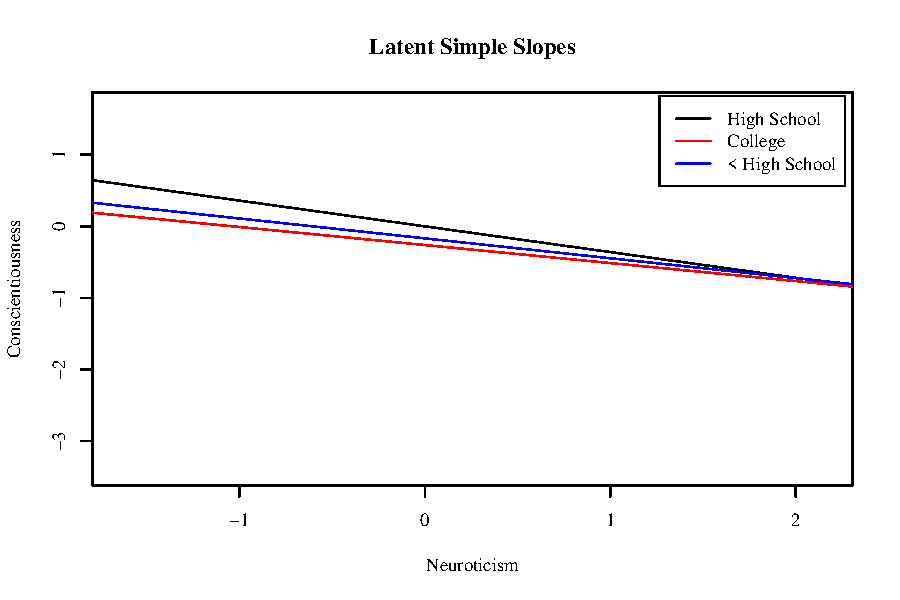
\includegraphics{sweaveFiles/-043}

\end{frame}


\end{document}
